\chapter{Data exploration and visualization}
\label{chap:R_data}

\epigraph{Clutter and confusion are failures of design, not attributes 
of information.}{\textit{Edward Tufte}}

Before you do any fancy statistical analyses with data, you must clean, 
explore, and visualize it. And eventually, you want to produce a 
finished product that presents visualizations you data and your results 
clearly and concisely. Ultimately, both, at the data exploration and the 
finished product stages, the goal of graphics is to present information 
such that it provides intuitive ideas. As Edward Tufte says: 
\begin{quote} \it
``Graphical excellence is that which gives to the viewer the greatest 
number of ideas in the shortest time with the least ink in the smallest 
space.'' 
\end{quote}

This chapter aims at introducing you to principles, and R packages and 
commands that will allow you to build a computational pipeline/workflow 
for critical steps of your data analysis and visualization. 

We will start with some basic plotting and data exploration. Then, you 
will learn to generate publication-quality graphics using the {\tt 
ggplot2} package. Finally, you will learn some principles and methods 
for data processing and storage in R. 

\section{Basic plotting and graphical data exploration}

R can produce beautiful graphics without the time-consuming and fiddly 
methods that you might have used in Excel or equivalent. You should 
also make it a habit to quickly plot the data for exploratory analysis. 
So we are going to learn some basic plotting first. 

\subsection{Basic plotting commands} 

Here is a menu of basic R plotting commands (use {\tt ?commandname} to 
learn more about it):

\begin{tabular}{p{3.1cm} p{10cm}} 
{\tt plot(x,y)} & Scatterplot\\
{\tt plot(y$\sim$x)} & Scatterplot with {\tt y} as a response variable \\
{\tt hist(mydata)} & Histogram\\
{\tt barplot(mydata)} & Bar plot\\
{\tt points(y1$\sim$x1)} & Add another series of points\\
{\tt boxplot(y$\sim$x)} & Boxplot\\
\end{tabular}\\

\subsection{R graphics devices}

In all that follows, you may often end up plotting multiple plots on 
the same graphics window without intending to do so, because R by 
default keeps plotting in the most recent plotting window that was 
opened. You can close a particular graphics window or "device" by using 
{\tt dev.off()}, and all open devices/windows with {\tt 
graphics.off()}. By default, {\tt dev.off()} will close the most recent 
figure device that was opened. 

\begin{tipbox}
Note that there are invisible devices in {\tt R}! Fore example, if you are 
	printing to pdf (coming up below), the device or graphics window will 
	not be visible on your computer screen. 
\end{tipbox}

Now let's try some simple plotting for data exploration. As a 
case study, we will use a dataset on Consumer-Resource (e.g., 
Predator-Prey) body mass ratios taken from the Ecological Archives of 
the ESA (Barnes {\em et al.} 2008, Ecology 89:881).

\begin{compactitem}[$\quad\star$]
	\item Copy the file {\tt EcolArchives-E089-51-D1.csv} from {\tt Data} directory in the master git repository on bitbucket to your own {\tt Data} directory. 
	\item Now, launch R and read in these data to a data frame:
\begin{lstlisting}
> MyDF <- read.csv("../Data/EcolArchives-E089-51-D1.csv")
> dim(MyDF) #check the size of the data frame you loaded
[1] 34931    15
\end{lstlisting}
\end{compactitem}

Let's look at what the data contain (type {\tt MyDF\$} and hit the TAB 
key twice (if you are using RStudio, you just can hit it once). This will give the following result: 
\begin{lstlisting}
> MyDF$
MyDF$Record.number                MyDF$Predator.mass
MyDF$In.refID                     MyDF$Prey
MyDF$IndividualID                 MyDF$Prey.common.name
MyDF$Predator                     MyDF$Prey.taxon
MyDF$Predator.common.name         MyDF$Prey.mass
MyDF$Predator.taxon               MyDF$Prey.mass.unit
MyDF$Predator.lifestage           MyDF$Location
MyDF$Type.of.feeding.interaction  
\end{lstlisting}
{\bf In RStudio, you will see a drop-down list of all the column 
headers when you hit {\tt tab}}.

You can also use the {\tt str()} and {\tt head()} commands that you 
learned about in Chapter \ref{chap:RI}.

As you can see, these data contain predator-prey body size information. 
This is an interesting dataset because it is huge, and covers a wide 
range of body sizes of aquatic species involved in consumer-resource 
interactions --- from unicells to whales. Analyzing this dataset should 
tell us a lot about what sizes of prey predators like to eat.

\begin{figure} \centering
   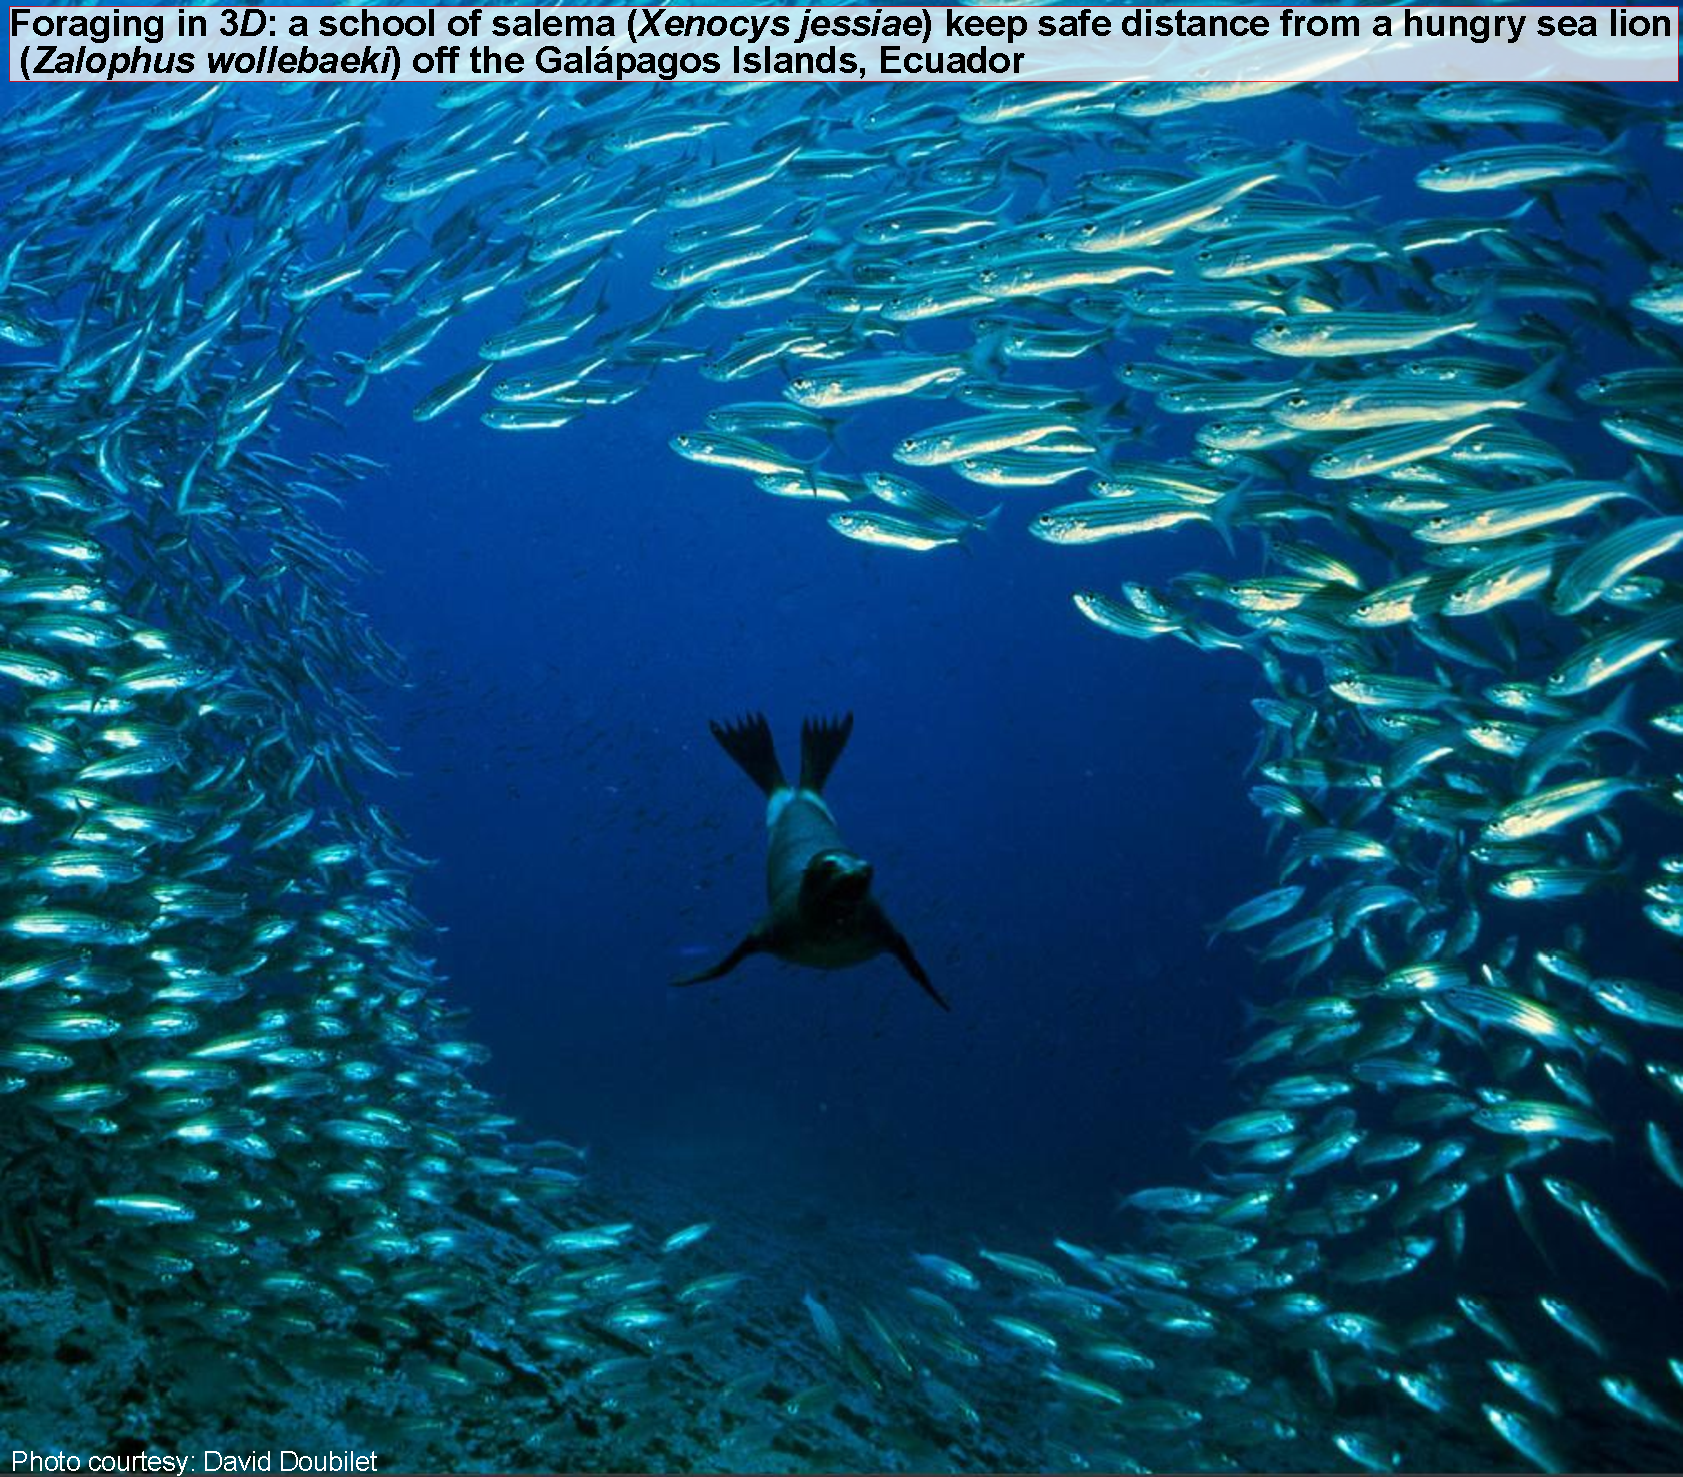
\includegraphics[width=0.8\textwidth]{SeaLion.pdf} 
	 \caption{A consumer-resource (predator-prey) interaction waiting to 
	 happen.}
\end{figure}

\subsection{Scatter Plot}

Let's start by plotting Predator mass vs. Prey mass:
\begin{lstlisting}
> plot(MyDF$Predator.mass,MyDF$Prey.mass)
\end{lstlisting}
\begin{center}
   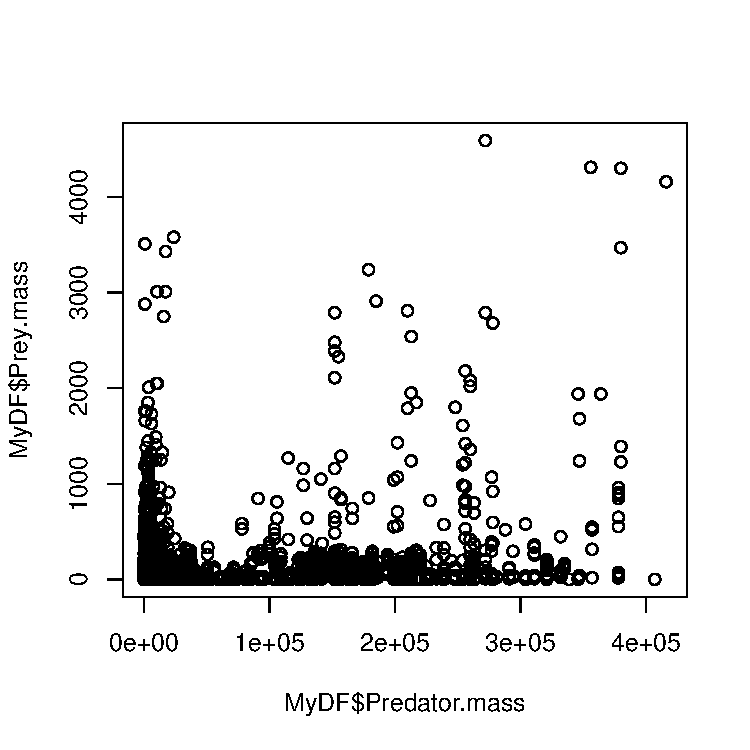
\includegraphics[width=0.5\textwidth]{PPScat1.pdf} 
\end{center}

That doesn't look very nice! Let's try taking logarithms (why?). 

\begin{lstlisting}
> plot(log(MyDF$Predator.mass),log(MyDF$Prey.mass))
\end{lstlisting}
\begin{center}
   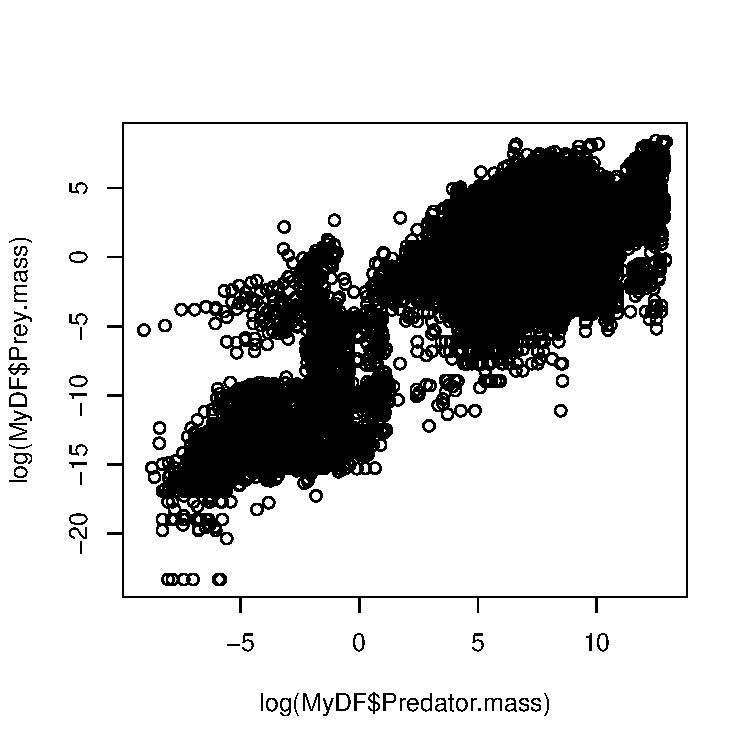
\includegraphics[width=0.5\textwidth]{PPScat2.pdf} 
\end{center}
We can change almost any aspect of the resulting graph; let's change the
symbols by specifying the {\tt p}lot {\tt ch}aracters using {\tt pch}:

\begin{lstlisting}
> plot(log(MyDF$Predator.mass),log(MyDF$Prey.mass),pch=20) # Change marker
\end{lstlisting}
\begin{center}
   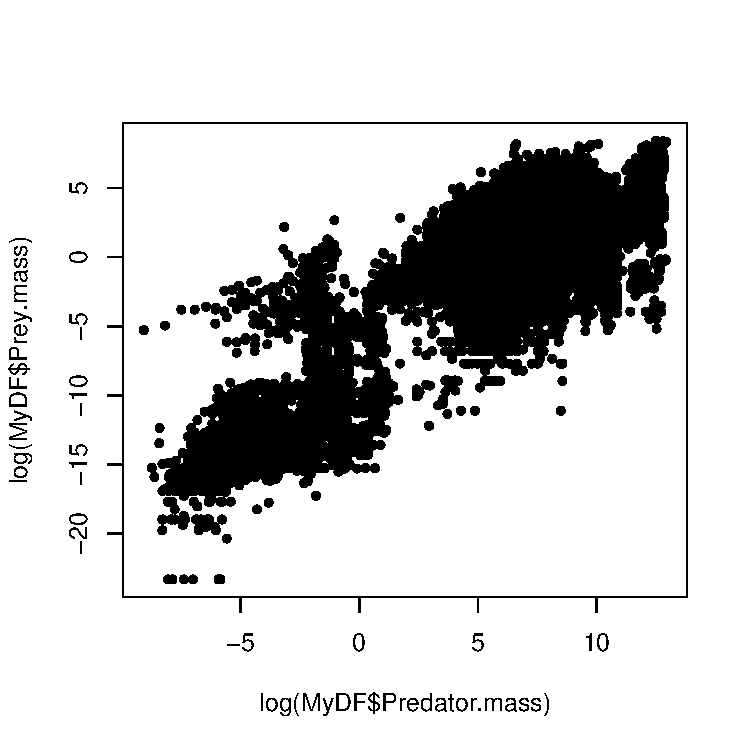
\includegraphics[width=0.5\textwidth]{PPScat3.pdf} 
\end{center}

\begin{lstlisting}
> plot(log(MyDF$Predator.mass),log(MyDF$Prey.mass),pch=20,
    xlab = "Predator Mass (kg)", ylab = "Prey Mass (kg)") # Add labels
\end{lstlisting}
\begin{center}
   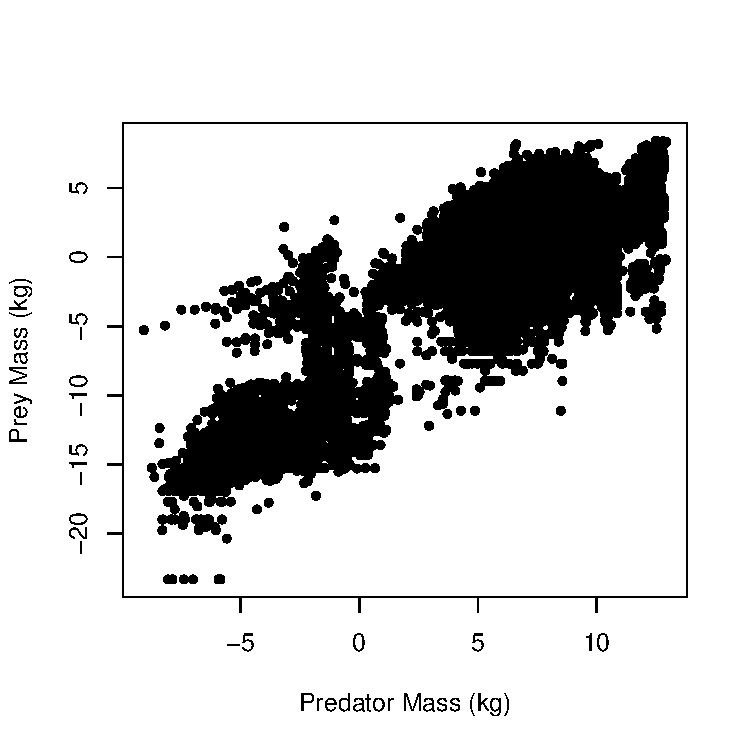
\includegraphics[width=0.5\textwidth]{PPScat4.pdf} 
\end{center}

\begin{tipbox}
	A really great summary of basic R graphical parameters can be found 
	at \url{https://www.statmethods.net/advgraphs/parameters.html}
\end{tipbox}

\subsection{Histograms}
Why did we have to take a logarithm to see the relationship between 
predator and prey size? Plotting histograms of the two classes 
(predator, prey) should be insightful, as we can then see the 
``marginal'' distributions of the two variables. 

Let's first plot a histogram of predator body masses:
\begin{lstlisting}
> hist(MyDF$Predator.mass)
\end{lstlisting}
\begin{center}
   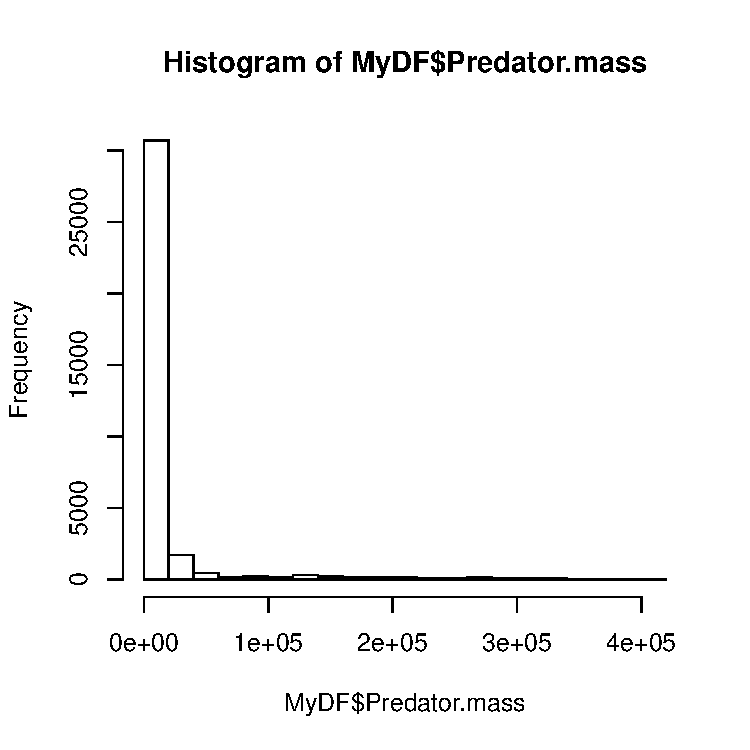
\includegraphics[width=0.5\textwidth]{PrHist1.pdf} 
\end{center}

Clearly, the data are heavily right skewed, with small body sized organisms 
dominating (that's a universal pattern on planet earth). Let's now take 
a logarithm and see if we can get a better idea of what the 
distribution of predator sizes looks like:
\begin{lstlisting}
> hist(log(MyDF$Predator.mass), 
   xlab = "Predator Mass (kg)", ylab = "Count") # include labels
\end{lstlisting}
\begin{center}
   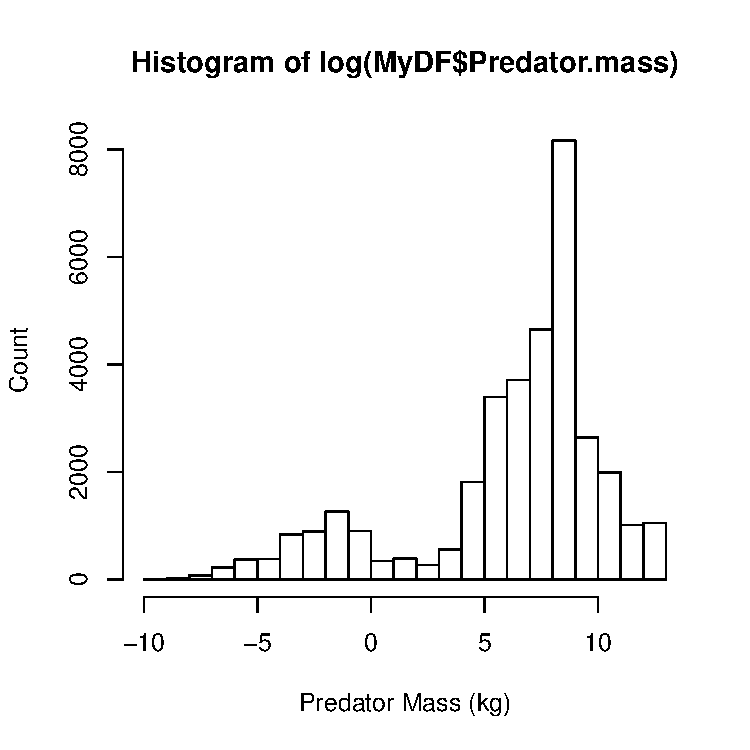
\includegraphics[width=0.5\textwidth]{PrHist2.pdf} 
\end{center}

\begin{lstlisting}
> hist(log(MyDF$Predator.mass),xlab="Predator Mass (kg)",ylab="Count", 
    col = "lightblue", border = "pink") # Change bar and borders colors 
\end{lstlisting}
\begin{center}
   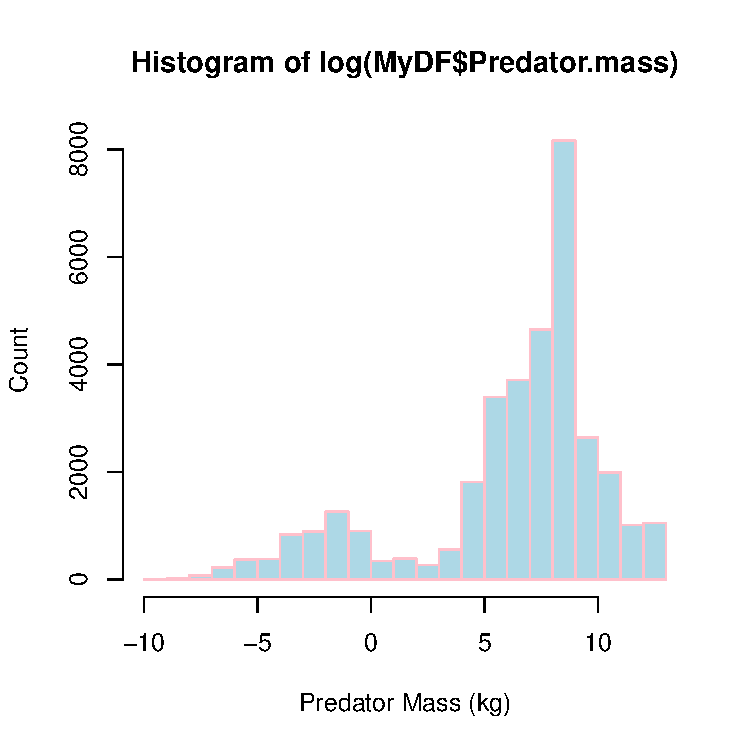
\includegraphics[width=0.5\textwidth]{PrHist3.pdf} 
\end{center}

So, taking a log really makes clearer what the distribution of body 
predator sizes looks like. {\it Try the same with prey body masses.}

\subsubsection{Exercise}

We can do a lot of beautification and fine-tuning of your R plots! As 
an exercise, try adjusting the histogram bin widths to make them same 
for the predator and prey, and making the x and y labels larger and in 
boldface. To get started, look at the help documentation of {\tt hist}.

\subsection{Subplots}
We can also plot both predator and prey body masses in different 
sub-plots using {\tt par} so that we can compare them visually. 

\begin{lstlisting}
> par(mfcol=c(2,1)) #initialize multi-paneled plot
> par(mfg = c(1,1)) # specify which sub-plot to use first 
> hist(log(MyDF$Predator.mass),
    xlab = "Predator Mass (kg)", ylab = "Count", 
    col = "lightblue", border = "pink", 
    main = 'Predator') # Add title
> par(mfg = c(2,1)) # Second sub-plot
> hist(log(MyDF$Prey.mass),
    xlab="Prey Mass (kg)",ylab="Count", 
    col = "lightgreen", border = "pink", 
    main = 'prey')
\end{lstlisting}
\begin{center}
   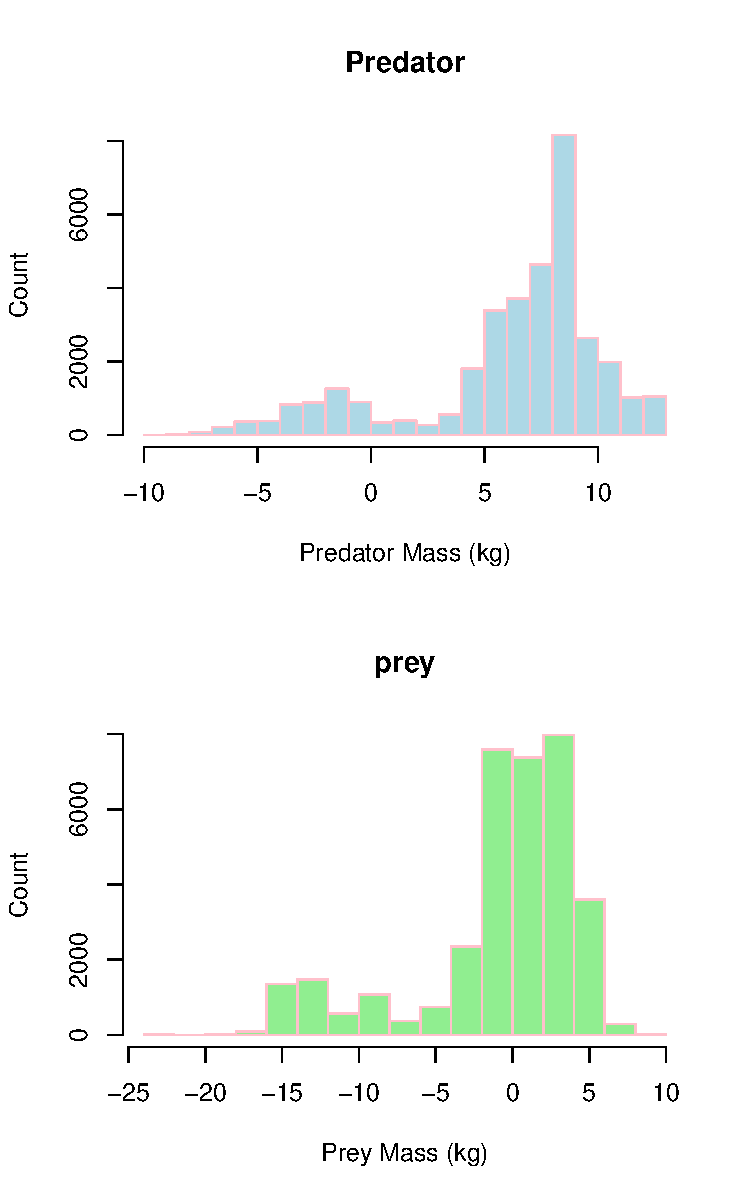
\includegraphics[width=0.5\textwidth]{PPHist1.pdf} 
\end{center}

Another option for making multi-panel plots is the {\tt layout} 
function. 

\subsection{Overlaying plots}
Better still, we would like to see if the predator mass and prey mass 
distributions are similar by overlaying them. 

\begin{lstlisting}
> hist(log(MyDF$Predator.mass), # Predator histogram
    xlab="Body Mass (kg)", ylab="Count", 
    col = rgb(1, 0, 0, 0.5), # Note 'rgb', fourth value is transparency
    main = "Predator-prey size Overlap") 
> hist(log(MyDF$Prey.mass), col = rgb(0, 0, 1, 0.5), add = T) # Plot prey
> legend('topleft',c('Predators','Prey'),   # Add legend
    fill=c(rgb(1, 0, 0, 0.5), rgb(0, 0, 1, 0.5))) # Define legend colors
\end{lstlisting}

\begin{tipbox}
	Plot annotation with text can be done with either single or double 
	quotes, i.e., `Plot Title' or ``Plot Title'', respectively. But it is generally a 
	good idea to use double quotes because sometimes you would like to 
	use an apostrophe in your title or axis label strings.   
\end{tipbox}

\begin{center}
   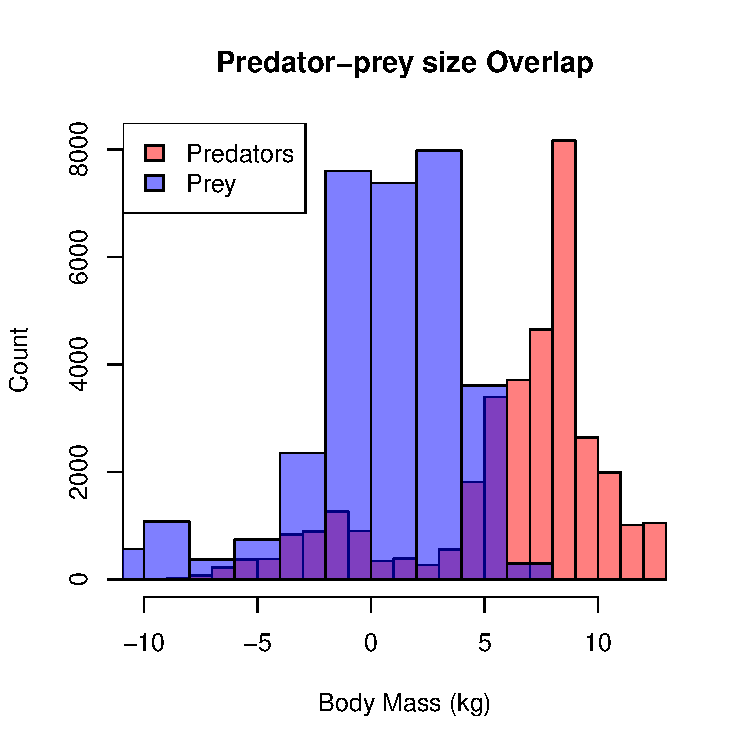
\includegraphics[width=0.5\textwidth]{PPOverlay.pdf} 
\end{center}

{\it It would be nicer to have both the plots with the same bin sizes 
-- try to do it}

\subsection{Boxplots}
Now, let's try plotting boxplots instead of  histograms. These are 
useful for getting a visual summary of the distribution of your data. 

\begin{lstlisting}
> boxplot(log(MyDF$Predator.mass),
	xlab = "Location", ylab = "Predator Mass",
	main = "Predator mass")
\end{lstlisting}
\begin{center}
   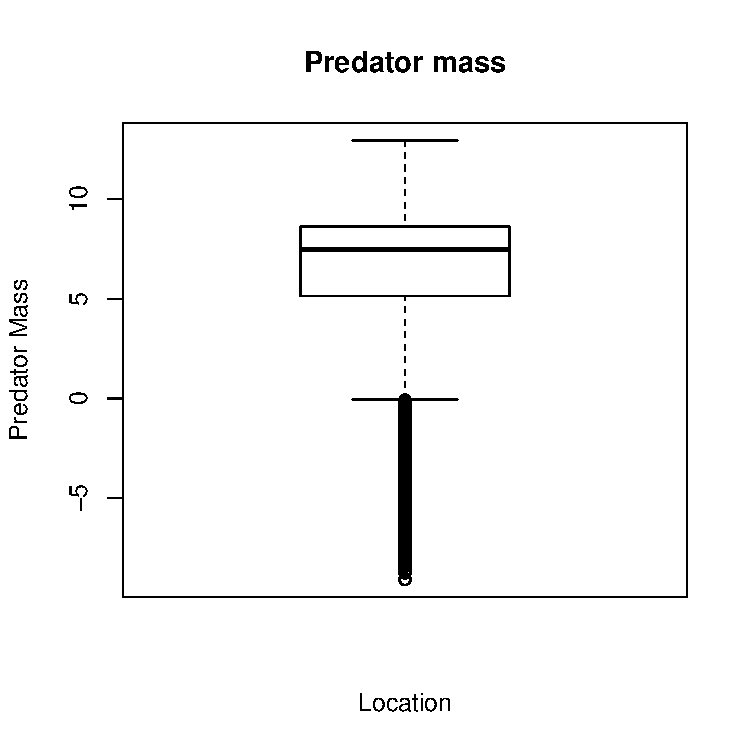
\includegraphics[width=0.5\textwidth]{PredBoxP1.pdf} 
\end{center}

Now let's see how many locations the data are from: 
\begin{lstlisting}
> boxplot(log(MyDF$Predator.mass) ~ MyDF$Location, # Why the tilde?
	xlab = "Location", ylab = "Predator Mass",
	main = "Predator mass by location")
\end{lstlisting}
\begin{center}
   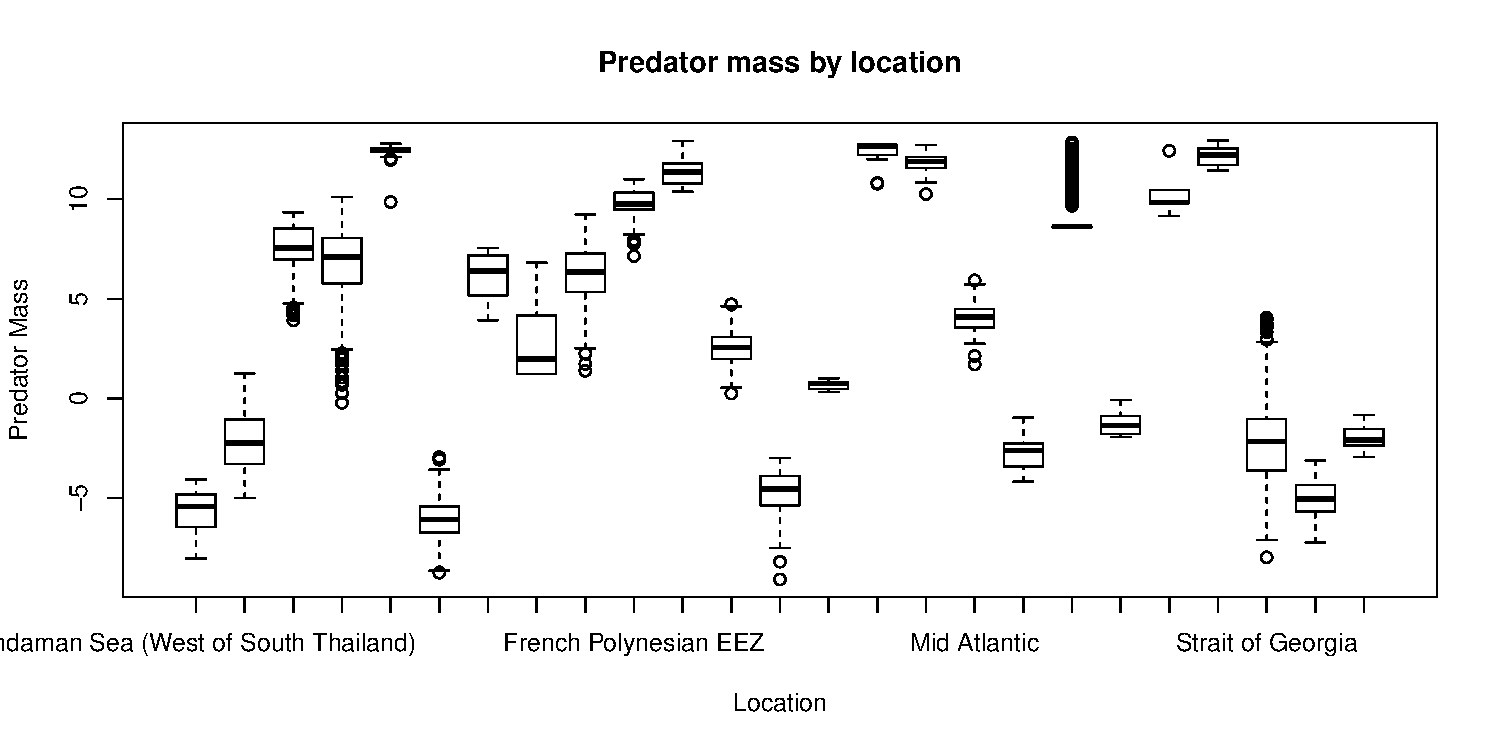
\includegraphics[width=1\textwidth]{PredBoxP2.pdf} 
\end{center}

Note the tilde (\textasciitilde). This is to tell R to subdivide or 
categorize your analysis and plot by the "Factor" location. More on 
this later. 

That's a lot of locations! You will need an appropriately wide plot to 
see all the boxplots adequately. Now let's try boxplots by feeding 
interaction type: 
\begin{lstlisting}
> boxplot(log(MyDF$Predator.mass) ~ MyDF$Type.of.feeding.interaction,
	xlab = "Location", ylab = "Predator Mass",
	main = "Predator mass by feeding interaction type")
\end{lstlisting}

\subsection{Combining plot types}

It would be nice to see both the predator and prey marginal 
distributions as well as the scatterplot for an exploratory analysis. 
We can do this by adding boxplots of the marginal variables to the scatterplot. 

\begin{lstlisting}
> par(fig=c(0,0.8,0,0.8)) # specify figure size as proportion
> plot(log(MyDF$Predator.mass),log(MyDF$Prey.mass),
    xlab = "Predator Mass (kg)", ylab = "Prey Mass (kg)") # Add labels
> par(fig=c(0,0.8,0.55,1), new=TRUE)
> boxplot(log(MyDF$Predator.mass), horizontal=TRUE, axes=FALSE)
> par(fig=c(0.65,1,0,0.8),new=TRUE)
> boxplot(log(MyDF$Prey.mass), axes=FALSE)
> mtext("Fancy Predator-prey scatterplot", side=3, outer=TRUE, line=-3)
\end{lstlisting}

\begin{center}
   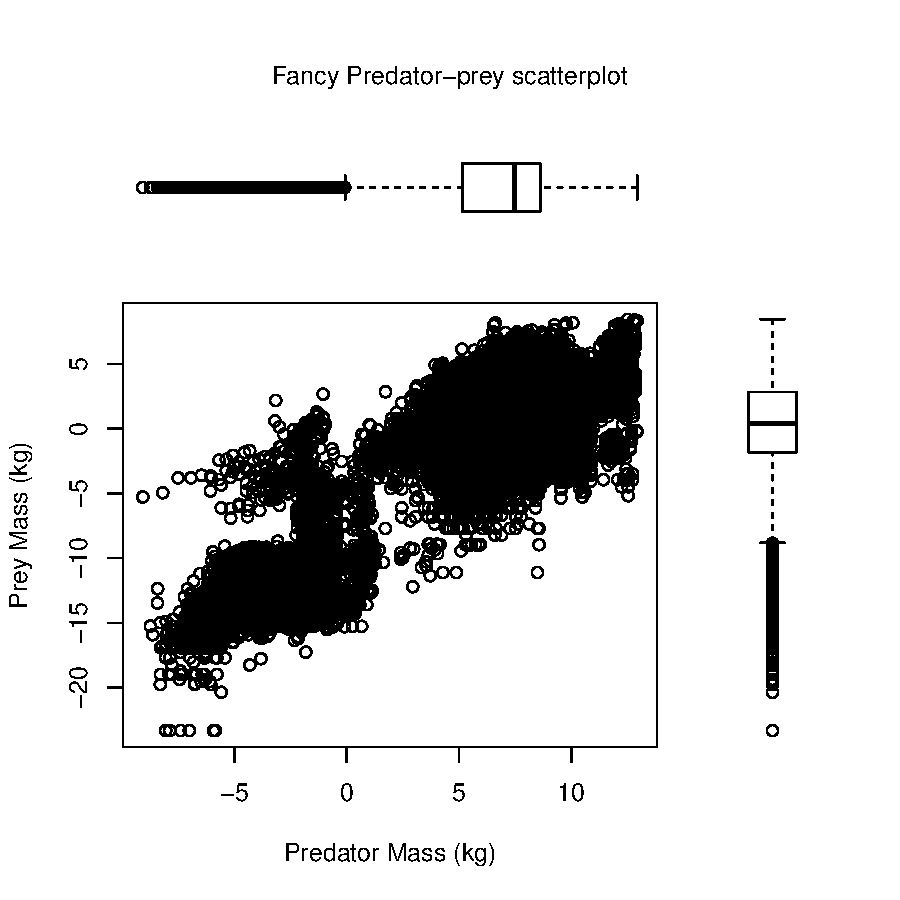
\includegraphics[width=0.6\textwidth]{PPScatFancy.pdf} 
\end{center}
To understand this plotting method, think of the full graph area as 
going from (0,0) in the lower left corner to (1,1) in the upper right 
corner. The format of the {\tt fig=} parameter is a numerical vector of 
the form {\tt c(x1, x2, y1, y2)}. The first {\tt fig= } sets up the 
scatterplot going from 0 to 0.8 on the x axis and 0 to 0.8 on the y 
axis. The top boxplot goes from 0 to 0.8 on the x axis and 0.55 to 1 on 
the y axis. The right hand boxplot goes from 0.65 to 1 on the x axis 
and 0 to 0.8 on the y axis. You can experiment with these proportions 
to change the spacings between plots.

\subsection{Lattice plots}
You can also make lattice graphs to avoid the somewhat laborious {\tt 
par()} approach above of getting multi-panel plots. For this, you will 
need to "load" a "library" that isn't included by default when you run 
R: 

\begin{lstlisting}
> library(lattice)
\end{lstlisting}

\begin{figure}
\centering
	\label{Fig-Lattice-1}
	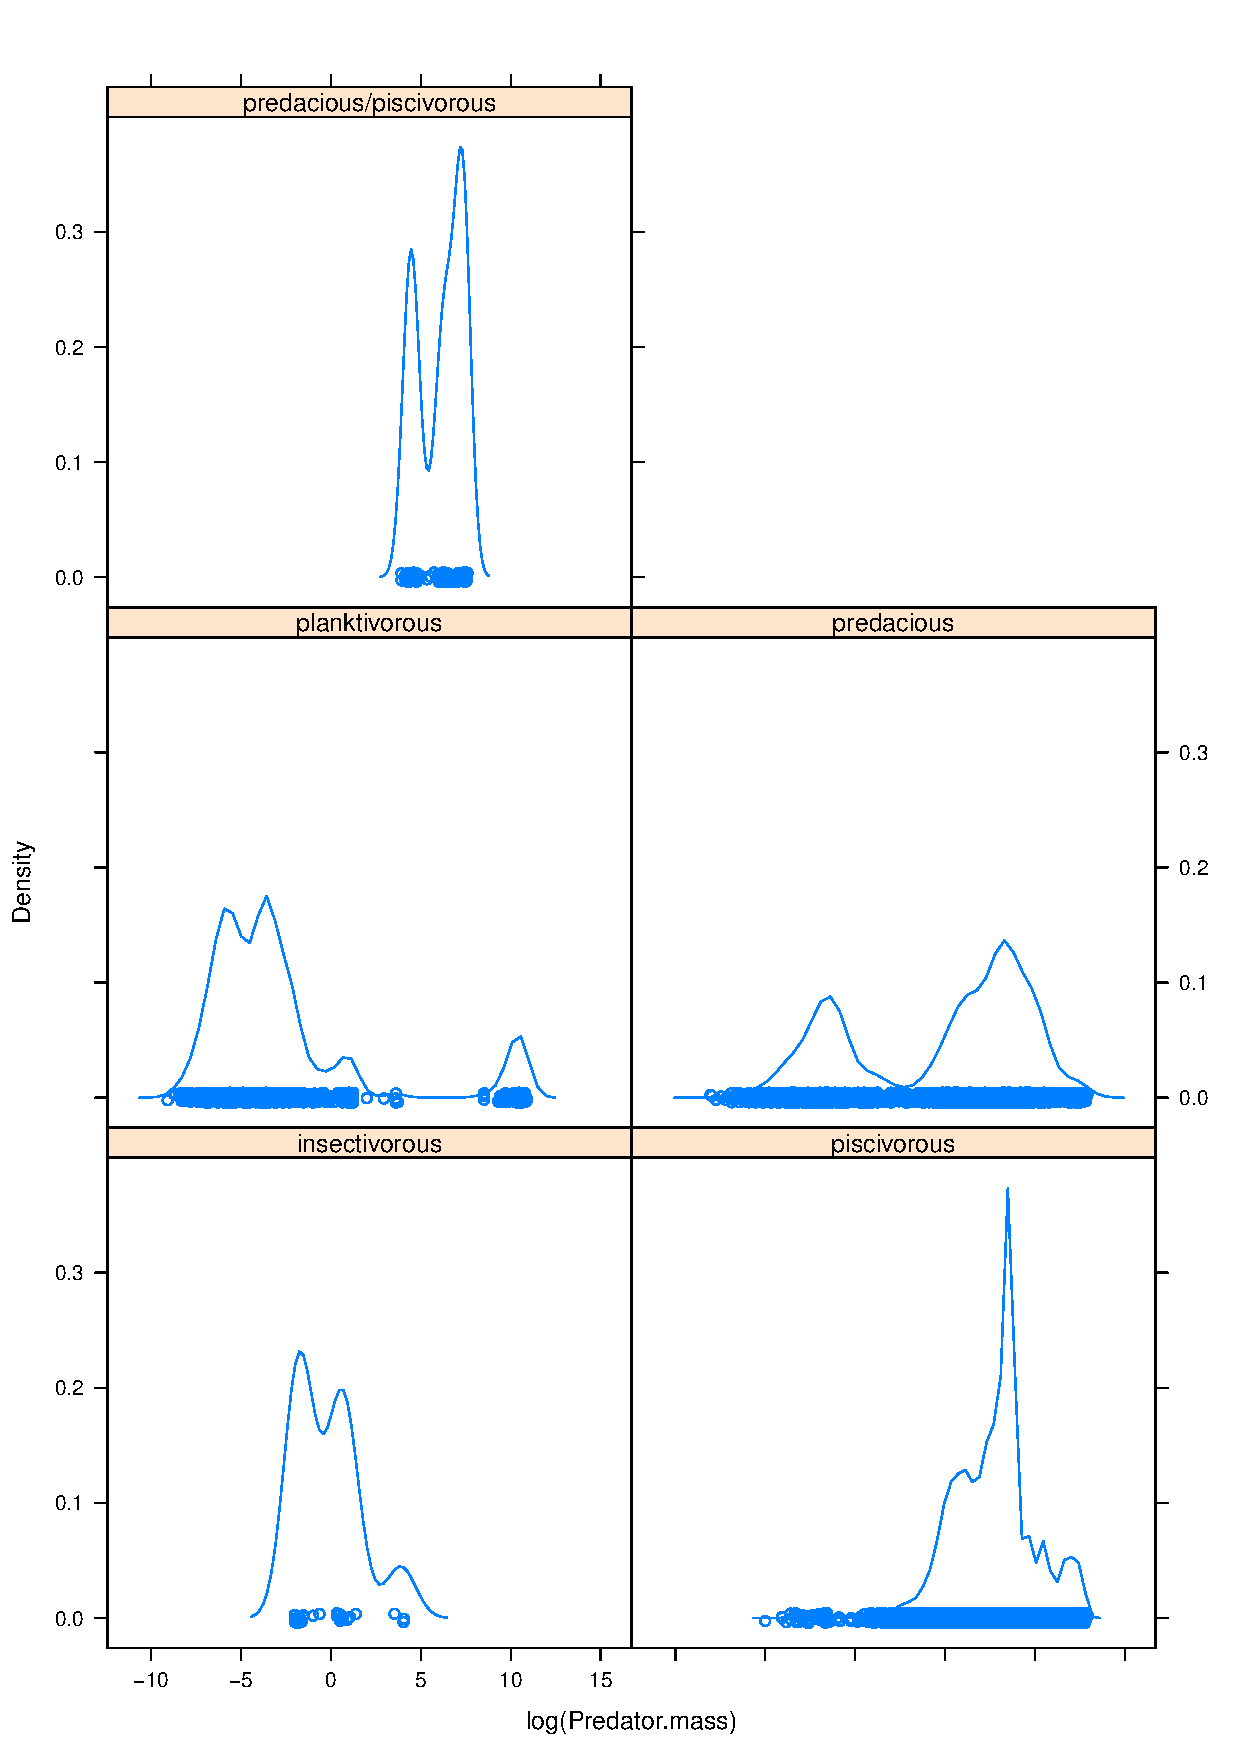
\includegraphics[width = 1 \linewidth]{PP_Lattice.pdf}
	\caption{A {\tt lattice} representation of the predator size data}
\end{figure}

A lattice plot of the above data for predator mass could look like Fig. 
\ref{Fig-Lattice-1} (as a density plot). This was generated using (and 
printing to a pdf with particular dimensions):

\begin{lstlisting}
> densityplot(~log(Predator.mass) | Type.of.feeding.interaction, 
data=MyDF)
\end{lstlisting}

Look up \url{http://www.statmethods.net/advgraphs/trellis.html} and the 
{\tt lattice} package help.

\subsection{Saving your graphics}

And you can also save the figure in a vector graphics format like a 
pdf. It is important to learn to do this, because you want to be able 
to save your plots in good resolution, and want to avoid the manual 
steps of clicking on the figure, doing "save as", etc. So let's 
save the figure as a PDF:  
\begin{lstlisting}
> pdf("../Results/Pred_Prey_Overlay.pdf", # Open blank pdf page 
    11.7, 8.3) # These numbers are page dimensions in inches
> hist(log(MyDF$Predator.mass), # Plot predator histogram (note 'rgb')
    xlab="Body Mass (kg)", ylab="Count", 
    col = rgb(1, 0, 0, 0.5), 
    main = "Predator-Prey Size Overlap") 
> hist(log(MyDF$Prey.mass), # Plot prey weights
    col = rgb(0, 0, 1, 0.5), 
    add = T)  # Add to same plot = TRUE
> legend('topleft',c('Predators','Prey'), # Add legend
    fill=c(rgb(1, 0, 0, 0.5), rgb(0, 0, 1, 0.5))) 
> dev.off() 
\end{lstlisting}

\begin{tipbox}
	Always try to save results in a vector format, which can be scaled up 
	to any size. For more on vector vs raster images/graphics, see: 
	\url{https://en.wikipedia.org/wiki/Vector_graphics}.
\end{tipbox}
Note that you are saving to the {\tt Results} directory now. This 
should always be your workflow: store and retrieve data from a {\tt 
Data} directory, keep your code and work from a {\tt Code} directory, 
and save outputs to a {\tt Results} directory.

You can also try other graphic output formats. For example, {\tt png()} 
(a raster format) instead of {\tt pdf()}. As always, look at the help 
documentation of each of these commands! 

\section{Practicals}
In this practical, you will write script that draws and saves three 
lattice graphs by feeding interaction type: one of predator mass, one 
of prey mass and one of the size ratio of prey mass over predator mass. 
Note that you would want to use logarithms of masses (or mass-ratios) 
for all three plots. In addition, the script will calculate the mean 
and median predator mass, prey mass and predator-prey size-ratios to a 
csv file. So:

\begin{compactitem}[$\quad\star$]
	
	\item Write a script file called {\tt PP\_Lattice.R} and save it in 
	the {\tt Code} directory --- sourcing or running this script should 
	result in three files called {\tt Pred\_Lattice.pdf}, {\tt 
	Prey\_Lattice.pdf}, and {\tt SizeRatio\_Lattice.pdf} being saved in 
	the {\tt Results} directory (the names are self-explanatory, I 
	hope).
    
	\item In addition, the script should calculate the mean and median 
	log predator mass, prey mass, and predator-prey size ratio, {\it by 
	feeding type}, and save it as a single csv output table called	{\tt 
	PP\_Results.csv} to the {\tt Results} directory. The table should 
	have appropriate headers (e.g., Feeding type, mean, median). (Hint: 
	you will have to initialize a new dataframe in the script to first 
	store the calculations) 

	\item The script should be self-sufficient and not need any 
	external inputs --- it should import the above predator-prey 
	dataset from the appropriate directory, and save the graphic plots 
	to the appropriate directory (Hint: use relative paths!).
	
	\item There are multiple ways to do this practical. The plotting and 
	saving component is simple enough. For calculating the statistics by 
	feeding type, you can either use the "loopy" way --- first obtaining 
	a list of feeding types (look up the {\tt unique} or {\tt levels} 
	functions) and then loop over them, using {\tt subset} to extract the 
	dataset by feeding type at each iteration, or the R-savvy way, by 
	using {\tt tapply} or {\tt ddply} and avoiding looping altogether 
	(Chapter \ref{chap:R_II}).
	
\end{compactitem}

%%%%%%%%%%%%%%%%%%%%%%%%%%%%%%%%%%%%%%%%%%%%%%%%%%%%%%%%%%%%%%%%%%%
%%%%%%%%%%%%%%%%%%%%%%%%%%%%%%%%%%%%%%%%%%%%%%%%%%%%%%%%%%%%%%%%%%%

\section{Publication-quality figures in R}

{\tt R} can produce beautiful graphics, but it takes a lot of work to 
obtain the desired result. This is because the starting point is pretty 
much a ``bare'' plot, and adding features commonly required for 
publication-grade figures (legends, statistics, regressions, etc.) can 
be quite involved. 
	
Moreover, it is very difficult to switch from one representation of the 
data to another (i.e., from boxplots to scatterplots), or to plot 
several datasets together. The {\tt R} package {\tt ggplot2} overcomes 
these issues, and produces truly high-quality, publication-ready 
graphics suitable for papers, theses and reports. 

\begin{tipbox}
Currently, {\tt ggplot2} cannot be used to create 3D graphs or mosaic 
plots. In any case, most of you won't be needing 3D plots! If you do, 
there are many ways to do 3D plots using other plotting packages in R. 
In particular, look up the {\tt scatterplot3d} and {\tt plot3D} 
packages.
\end{tipbox}

% \section{Fundamental rules of visualization}

% \begin{compactitem}

	% \item Make sure the text within the figure and outside on the axes ad 
	% labels will be visible at about once you rescale the figure to its 
	% final size. 
	
	% \item Be careful about reds and greens --- as many as 10\% of men can 
	% be color-blind!
	
	% \item Use vector, not raster graphics (to the extent possible)
	
% \end{compactitem}

{\tt ggplot2} differs from other approaches as it attempts to provide a 
``grammar'' for graphics in which each layer is the equivalent of a 
verb, subject etc. and a plot is the equivalent of a sentence. All 
graphs start with a layer showing the data, other layers and commands 
are added to modify the plot. Specifically, according to this grammar, 
a statistical graphic is a ``mapping'' from data to aesthetic 
attributes (colour, shape, size; set using {\tt aes}) of geometric 
objects (points, lines, bars; set using {\tt geom}).  

For more on the ideas underlying ggplot, see the book ``ggplot2: 
Elegant Graphics for Data Analysis'', by H. Wickham (in your Reading 
directory). Also, the website \url{ ggplot2.org} a great resource. 

{\tt ggplot2} should already be available on the college computers. If 
you are using your own computer, look up the section on installing 
packages in Chapter \ref{chap:RI}. 

ggplot can be used in two ways: with {\tt qplot} (for {\tt q}uick {\tt 
plot}ting) and {\tt ggplot} for full-blown, customizable plotting.

\begin{tipbox}
Note that {\tt ggplot2} only accepts data in data frames. 	
\end{tipbox}

\subsection{Basic plotting with {\tt qplot}}

{\tt qplot} can be used to quickly produce graphics for exploratory 
data analysis, and as a base for more complex graphics. It uses syntax 
that is closer to the standard R plotting commands. 

We will use the same predator-prey body size dataset again -- you will 
soon see how much nice the same types of plots you made above look when 
done with ggplot!. 

\subsubsection{Scatterplots}

Let's start plotting the {\tt Predator.mass} vs {\tt Prey.mass}:
\begin{lstlisting}
> require(ggplot2)  ## Load the package
Loading required package: ggplot2
> qplot(Prey.mass, Predator.mass, data = MyDF)
\end{lstlisting}

As before, let's take logarithms and plot:

\begin{lstlisting}
> qplot(log(Prey.mass), log(Predator.mass), data = MyDF)
\end{lstlisting}

Now, color the points according to the type of feeding interaction:

\begin{lstlisting}
> qplot(log(Prey.mass), log(Predator.mass), data = MyDF, 
	colour = Type.of.feeding.interaction)
\end{lstlisting}

The same as above, but changing the shape:
\begin{lstlisting}
> qplot(log(Prey.mass), log(Predator.mass), data = MyDF, 
	shape = Type.of.feeding.interaction)
\end{lstlisting}

\subsubsection{Aesthetic mappings}
These examples demonstrate a key difference between {\tt qplot} and the 
standard {\tt plot} command: When you want to assign colours, sizes or 
shapes to the points on your plot, using the {\tt plot} command, it's 
your responsibility to convert (i.e., ``map'') a categorical variable 
in your data (e.g., type of feeding interaction in the above case) onto 
colors (or shapes) that {\tt plot} knows how to use (e.g., by 
specifying ``red'', ``blue'', ``green'', etc). 

ggplot does this mapping for you automatically, and also provides a 
legend! This makes it really easy to quickly include additional data 
(e.g., if a new feeding interaction type was added to the data) on the 
plot. 

Instead of using ggplot's automatic mapping, if you want to  manually 
set a color or a shape, you have to use {\tt I()} (meaning 
``Identity''). To see this in practice, try the following:
\begin{lstlisting}
> qplot(log(Prey.mass), log(Predator.mass), 
	data = MyDF, colour = "red")
\end{lstlisting}
You chose red, but ggplot used mapping to convert it to a particular 
shade of red. To set it manually to the real red, do this:
\begin{lstlisting}
> qplot(log(Prey.mass), log(Predator.mass), 
	data = MyDF, colour = I("red"))
\end{lstlisting}

Similarly, for point size, compare these two:
\begin{lstlisting}
> qplot(log(Prey.mass), log(Predator.mass), 
	data = MyDF, size = 3) #with ggplot size mapping
> qplot(log(Prey.mass), log(Predator.mass), 
	data = MyDF, size = I(3)) #no mapping
\end{lstlisting}

But for shape, ggplot doesn't have a continuous mapping because shapes 
are a discrete variable. To see this, compare these two:
\begin{lstlisting}
> qplot(log(Prey.mass), log(Predator.mass), 
	data = MyDF, shape = 3) #will give error
> qplot(log(Prey.mass), log(Predator.mass), 
	data = MyDF, shape= I(3))
\end{lstlisting}

\subsubsection{Setting transparency}
Because there are so many points, we can make them semi-transparent 
using {\tt alpha} so that the overlaps can be seen:
\begin{lstlisting}
> qplot(log(Prey.mass), log(Predator.mass), data = MyDF, 
	colour = Type.of.feeding.interaction, alpha = I(.5))
\end{lstlisting}
Here try using {\tt alpha = .5} instead of {\tt alpha = I(.5)} and see 
what happens.

\subsubsection{Adding smoothers and regression lines}

Now add a smoother to the points: 
\begin{lstlisting}
> qplot(log(Prey.mass), log(Predator.mass), data = MyDF, 
	geom = c("point", "smooth"))
\end{lstlisting}

If we want to have a linear regression, we need to specify the method 
as being {\tt lm}:

\begin{lstlisting}
> qplot(log(Prey.mass), log(Predator.mass), data = MyDF, 
	geom = c("point", "smooth")) + geom_smooth(method = "lm")
\end{lstlisting}

{\tt lm} stands for {\tt l}inear {\tt m}odels (linear regression is a type 
of linear model). You will learn about linear models and fitting them 
to data (as you have done here) in the Stats in R week. 

We can also add a ``smoother'' for each type of interaction:
\begin{lstlisting}
> qplot(log(Prey.mass), log(Predator.mass), data = MyDF, 
	geom = c("point", "smooth"), colour = Type.of.feeding.interaction)  
				+ geom_smooth(method = "lm")
\end{lstlisting}

To extend the lines to the full range, use {\tt fullrange = TRUE}:

\begin{lstlisting}
> qplot(log(Prey.mass), log(Predator.mass), data = MyDF, 
	geom = c("point", "smooth"),
	colour = Type.of.feeding.interaction) + 
	geom_smooth(method = "lm",fullrange = TRUE)
\end{lstlisting}

Now we want to see how the ratio between prey and predator mass changes 
according to the type of interaction:

\begin{lstlisting}
> qplot(Type.of.feeding.interaction, 
		log(Prey.mass/Predator.mass), data = MyDF)
\end{lstlisting}

Because there are so many points, we can ``jitter'' them to get a
better idea of the spread:

\begin{lstlisting}
> qplot(Type.of.feeding.interaction, 
		log(Prey.mass/Predator.mass), data = MyDF,
		geom = "jitter")
\end{lstlisting}

\subsubsection{Boxplots}

Or we can draw a boxplot of the data (note the {\tt geom} argument, 
which stands for {\tt geom}etry):

\begin{lstlisting}
> qplot(Type.of.feeding.interaction, 
		log(Prey.mass/Predator.mass), data = MyDF,
		geom = "boxplot")
\end{lstlisting}

\subsubsection{Histograms and density plots}

Now let's draw an histogram of predator-prey mass ratios:

\begin{lstlisting}
> qplot(log(Prey.mass/Predator.mass), data = MyDF, 
	geom =  "histogram")
\end{lstlisting}

Color the histogram according to the interaction type:

\begin{lstlisting}
> qplot(log(Prey.mass/Predator.mass), data = MyDF, 
	geom =  "histogram", 
	fill = Type.of.feeding.interaction)
\end{lstlisting}

You may want to define binwidth (in units of x axis):

\begin{lstlisting}
> qplot(log(Prey.mass/Predator.mass), data = MyDF, 
	geom =  "histogram", 
	fill = Type.of.feeding.interaction,
	binwidth = 1)
\end{lstlisting}

To make it easier to read, we can plot the smoothed density of the 
data:

\begin{lstlisting}
> qplot(log(Prey.mass/Predator.mass), data = MyDF, 
	geom =  "density", fill = Type.of.feeding.interaction)
\end{lstlisting}

And you can make the densities transparent so that the overlaps are 
visible:

\begin{lstlisting}
> qplot(log(Prey.mass/Predator.mass), data = MyDF, 
	geom =  "density", fill = Type.of.feeding.interaction, alpha = 
	I(0.5))
\end{lstlisting}

Or using {\tt colour} instead of {\tt fill} draws only the edge of
the curve:
\begin{lstlisting}
> qplot(log(Prey.mass/Predator.mass), data = MyDF, 
	geom =  "density", colour = Type.of.feeding.interaction)
\end{lstlisting}

Similarly, {\tt geom = "bar"} produces a barplot, {\tt geom =
	"line"} a series of points joined by a line, etc.

\subsubsection{Multi-faceted plots}
An alternative way of displaying data belonging to different classes
is using ``faceting''. We did this using {\tt 
lattice()} previously, but ggplot does a much nicer job:

\begin{lstlisting}
> qplot(log(Prey.mass/Predator.mass), 
	facets = Type.of.feeding.interaction ~., 
	data = MyDF, geom =  "density")
\end{lstlisting}

The {\tt \textasciitilde .} (the space is not important) notation tells 
ggplot whether to do the faceting by row or by column. So if you want a 
by-column configuration, switch {\tt \textasciitilde} and {\tt .}, and 
also swap the position of the {\tt .\textasciitilde}:

\begin{lstlisting}
> qplot(log(Prey.mass/Predator.mass), 
	facets =  .~ Type.of.feeding.interaction, 
	data = MyDF, geom =  "density")
\end{lstlisting}

You can also facet by a combination of categories (this is going to be 
a big plot!):

\begin{lstlisting}
> qplot(log(Prey.mass/Predator.mass), 
	facets = .~ Type.of.feeding.interaction + Location, 
	data = MyDF, geom =  "density")
\end{lstlisting}

And you can also change the order of the combination:

\begin{lstlisting}
> qplot(log(Prey.mass/Predator.mass), 
	facets = .~ Location + Type.of.feeding.interaction, 
	data = MyDF, geom =  "density")
\end{lstlisting}

\begin{tipbox}
	For more fine-tuned faceting, look up the {\tt facet\_grid()} and 
	{\tt facet\_wrap()} functions within {\tt ggplot2}. look up \url{ 
	http://www.cookbook-r.com/Graphs/Facets_(ggplot2)}. 
	
	See Fig. \ref{PPRegress} for an example result. 
\end{tipbox}

\subsubsection{Logarithmic axes}
A more elegant way of drawing logarithmic quantities is to set the axes 
to be logarithmic:

\begin{lstlisting}
> qplot(Prey.mass, Predator.mass, data = MyDF, log="xy")
\end{lstlisting}

\subsubsection{Plot annotations}

Let's add a title and labels:

\begin{lstlisting}
> qplot(Prey.mass, Predator.mass, data = MyDF, log="xy",
	main = "Relation between predator and prey mass", 
	xlab = "log(Prey mass) (g)", 
	ylab = "log(Predator mass) (g)")
\end{lstlisting}

Adding {\tt + theme\_bw()} makes it suitable for black and white
printing.

\begin{lstlisting}
> qplot(Prey.mass, Predator.mass, data = MyDF, log="xy",
	main = "Relation between predator and prey mass", 
	xlab = "Prey mass (g)", 
	ylab = "Predator mass (g)") + theme_bw()
\end{lstlisting}

\subsubsection{Saving your plots}

Finally, let's save a pdf file of the figure (same approach as we used 
before):
\begin{lstlisting}
> pdf("../Results/MyFirst-ggplot2-Figure.pdf")
> print(qplot(Prey.mass, Predator.mass, data = MyDF,log="xy",
	main = "Relation between predator and prey mass", 
	xlab = "log(Prey mass) (g)", 
	ylab = "log(Predator mass) (g)") + theme_bw())
> dev.off()
\end{lstlisting}

Using {\tt print} ensures that the whole command is kept together and 
that you can use the command in a script.

\subsection{Some more important ggplot options}
Other important options to keep in mind:

\begin{tabular}{p{1.8cm} p{11cm}} 
	{\tt xlim} & limits for x axis: {\tt xlim = c(0,12)}\\
	{\tt ylim} & limits for y axis\\
	{\tt log} & log transform variable {\tt log = "x"},
		{\tt log = "y"}, {\tt log = "xy"}\\
	{\tt main} & title of the plot {\tt main = "My Graph"}\\
	{\tt xlab} & x-axis label\\
	{\tt ylab} & y-axis label\\
	{\tt asp} & aspect ratio  {\tt asp = 2}, {\tt asp = 0.5}\\
	{\tt margins} & whether or not margins will be displayed\\
\end{tabular}\\

\subsection{Various {\tt geom}}

{\tt geom} Specifies the geometric objects that define the graph type. 
The geom option is expressed as a character vector with one or more 
entries. geom values include "point", "smooth", "boxplot", "line", 
"histogram", "density", "bar", and "jitter". Try the following:

\lstinputlisting[language=R]{Practicals/Code/qplotExamples.R}

\subsection{Advanced plotting: {\tt ggplot}}

The command {\tt qplot} allows you to use only a single dataset and
a single set of ``aesthetics'' (x, y, etc.). To make full use of
{\tt ggplot2}, we need to use the command {\tt ggplot}, which allows 
you to use ``layering''. Layering is the mechanism by which additional 
data elements are added to a plot. Each layer can come from a different 
dataset and have a different aesthetic mapping, allowing us to create 
plots that could not be generated using {\tt qplot()}, which permits 
only a single dataset and a single set of aesthetic mappings. 

For a {\tt ggplot} plotting command, we need at least:
\begin{itemize}
	\item The data to be plotted, in a data frame;
	\item Aesthetics mappings, specifying which variables we want to
	plot, and how;
	\item The {\tt geom}, defining the geometry for representing the data;
	\item (Optionally) some {\tt stat} that transforms the data or
	performs statistics using the data.
\end{itemize}

To start a graph, we nust specify the data and the aesthetics:

\begin{lstlisting}
> p <- ggplot(MyDF, aes(x = log(Predator.mass),
				y = log(Prey.mass),
				colour = Type.of.feeding.interaction ))
\end{lstlisting}

Here we have created a graphics object {\tt p} to which we can add 
layers and other plot elements. 

Now try to plot the graph:

\begin{lstlisting}
> p
Error: No layers in plot
\end{lstlisting}

That is because we are yet to specify a geometry --- only then can we 
see the graph:

\begin{lstlisting}
> p + geom_point()
\end{lstlisting}

We can use the ``plus'' sign to concatenate different commands:

\begin{lstlisting}
> p <- ggplot(MyDF, aes(x = log(Predator.mass),
				y = log(Prey.mass),
				colour = Type.of.feeding.interaction ))
> q <- p + geom_point(size=I(2), shape=I(10)) + theme_bw()
> q
\end{lstlisting}

Let's remove the legend:

\begin{lstlisting}
> q + theme(legend.position = "none")
\end{lstlisting}

We will not look at some case studies to see some useful ways in which
you can use ggplot.

\subsection{Case study 1: plotting a matrix}
\begin{figure}
	\begin{center}
	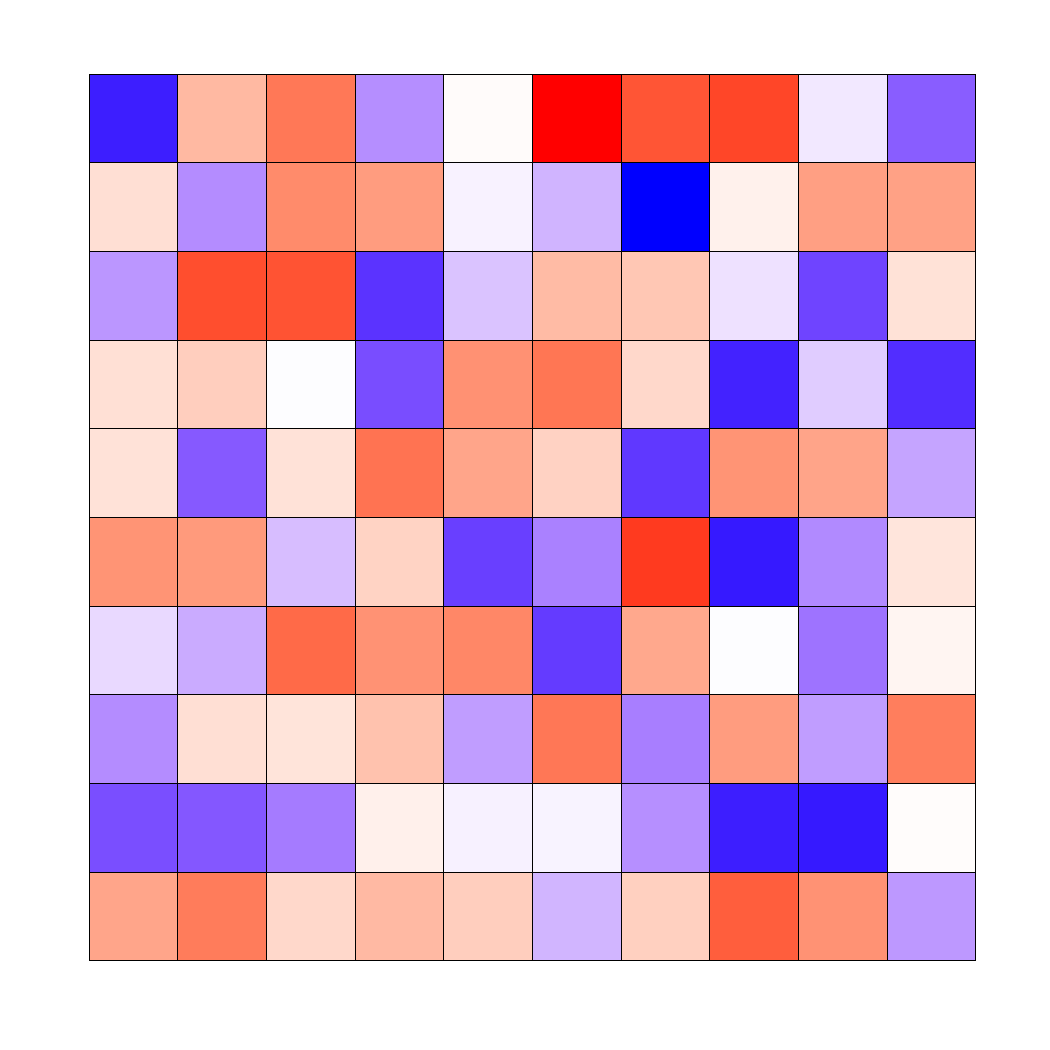
\includegraphics[width = 0.5 \linewidth]{FigureMatrix.pdf}
	\end{center}
	\caption{Random matrix with values sampled from uniform
	distribution.}
	\label{MatPlot}
\end{figure}

Here we will plot a matrix of random values taken from a normal 
distribution $\mathcal U [0,1]$. Our goal is to produce the plot in 
Figure \ref{MatPlot}. Because we want to plot a matrix, and {\tt 
ggplot2} accepts only dataframes, we use the package {\tt reshape2} 
that can ``melt'' a matrix into a dataframe:

\begin{lstlisting}
require(ggplot2)
require(reshape2)

GenerateMatrix <- function(N){
	M <- matrix(runif(N * N), N, N)
	return(M)
}

> M <- GenerateMatrix(10)

> M[1:3, 1:3]
			[,1]      [,2]      [,3]
[1,] 0.2700254 0.8686728 0.7365857
[2,] 0.1744879 0.8488169 0.4165879
[3,] 0.3980783 0.7727821 0.4271121

> Melt <- melt(M)

> Melt[1:4,]
  Var1 Var2     value
1    1    1 0.0698925
2    2    1 0.6333296
3    3    1 0.8990120
4    4    1 0.8425578

> ggplot(Melt, aes(Var1, Var2, fill = value)) + geom_tile()

# adding a black line dividing cells
> p <- ggplot(Melt, aes(Var1, Var2, fill = value))
> p <- p + geom_tile(colour = "black")

# removing the legend
> q <- p + theme(legend.position = "none")

# removing all the rest
> q <- p + theme(legend.position = "none", 
	 panel.background = element_blank(),
	 axis.ticks = element_blank(), 
	 panel.grid.major = element_blank(),
	 panel.grid.minor = element_blank(),
	 axis.text.x = element_blank(),
	 axis.title.x = element_blank(),
	 axis.text.y = element_blank(),
	 axis.title.y = element_blank())

# exploring the colors
> q + scale_fill_continuous(low = "yellow",
						high = "darkgreen")
> q + scale_fill_gradient2()
> q + scale_fill_gradientn(colours = grey.colors(10))
> q + scale_fill_gradientn(colours = rainbow(10))
> q + scale_fill_gradientn(colours =
				c("red", "white", "blue"))
\end{lstlisting}

% check if scale_fill_gradient2() is deprecated

\subsection{Case study 2: plotting two dataframes}

According to Girko's circular law, the eigenvalues of a matrix $M$ of
size $N \times N$ are approximately contained in a circle in the
complex plane with radius $\sqrt{N}$. We are going to draw a
simulation displaying this result (Figure \ref{Girko}).

\lstinputlisting[language=R]{Practicals/Code/Eigen.R}
\begin{figure}\centering
	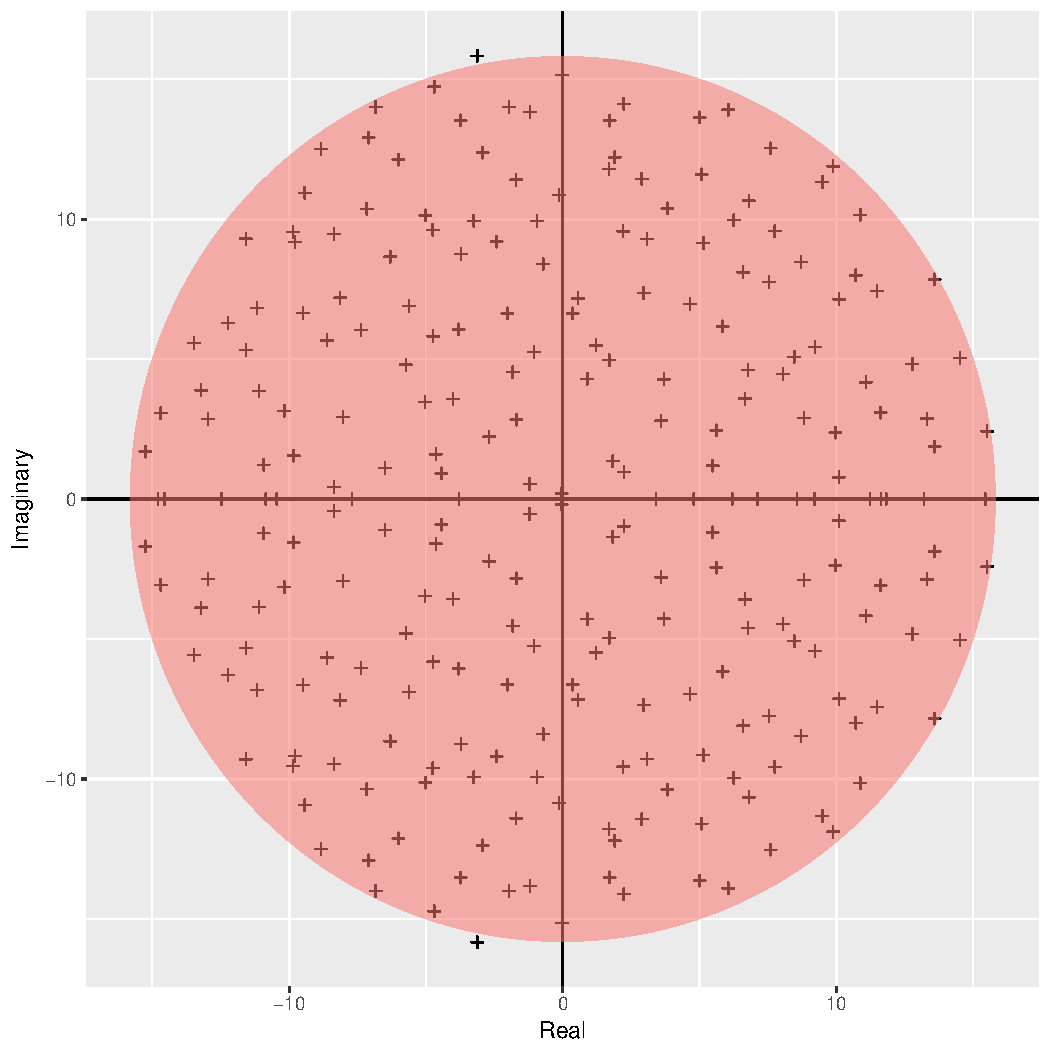
\includegraphics[width = 0.6\linewidth]{Girko.pdf}
	\caption{Girko's circular law.}
	\label{Girko}
\end{figure}

\subsection{Case study 3: annotating plots}

In the plot in Figure \ref{Linebar}, we use the geometry ``text'' to
annotate the plot.

\lstinputlisting[language=R]{Practicals/Code/bars.R}
\begin{figure}
	\begin{center}
	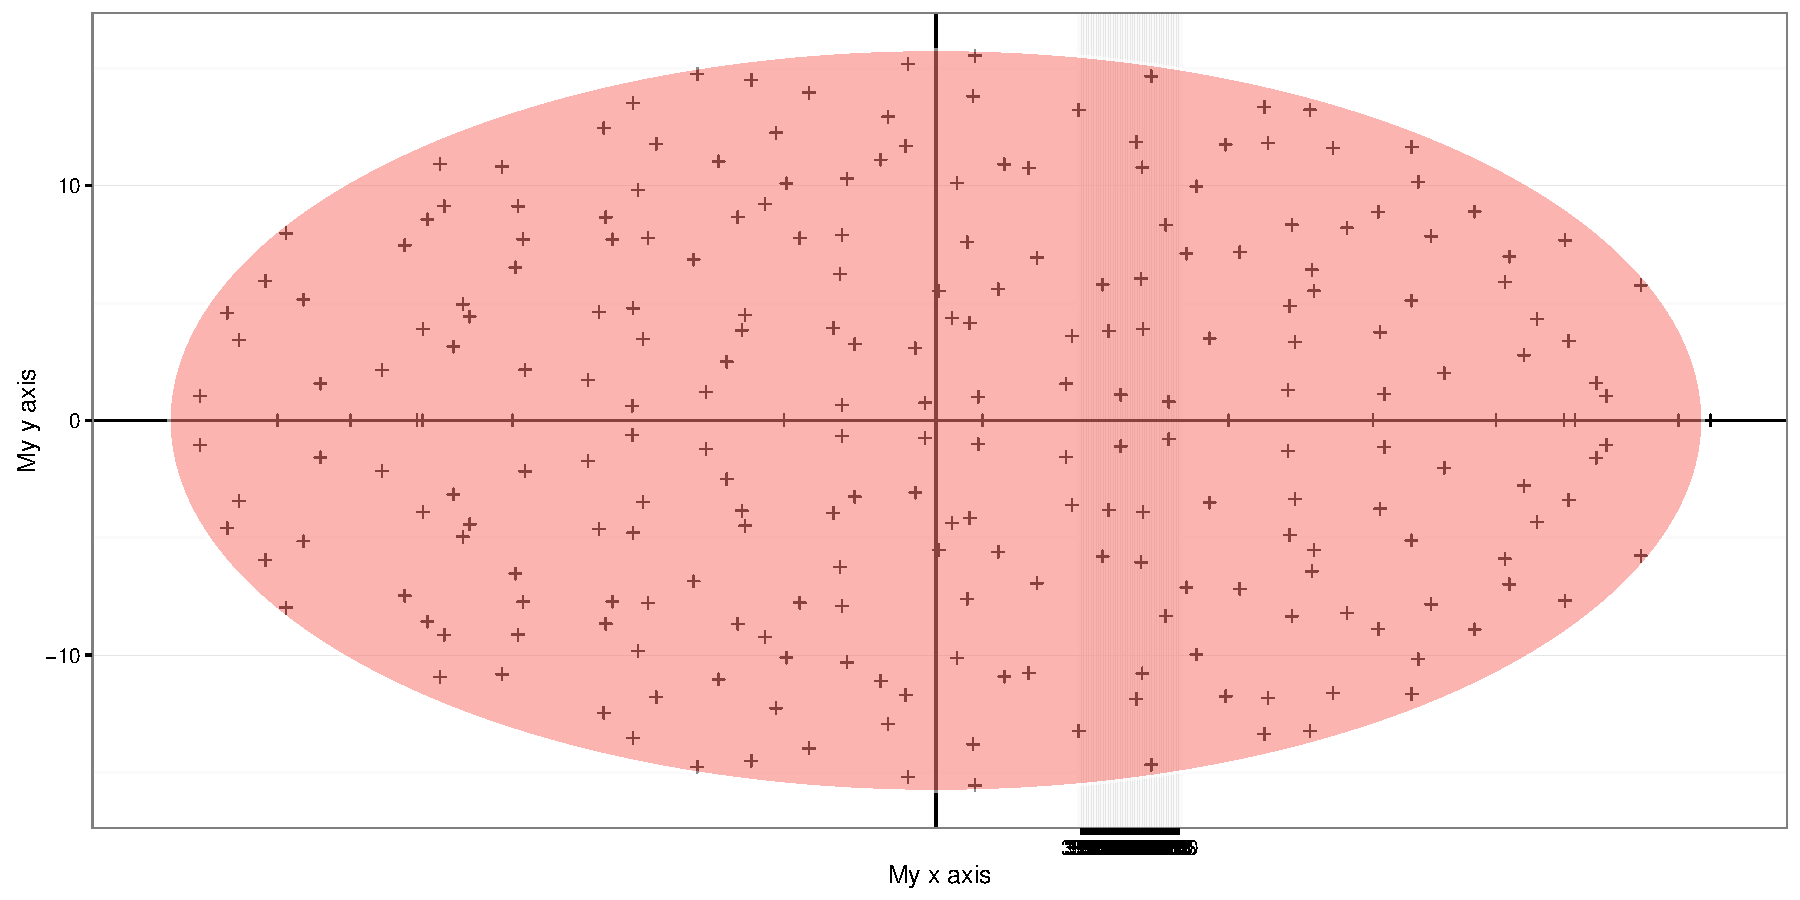
\includegraphics[width = \linewidth]{MyBars.pdf}
	\end{center}
	\caption{Overlay of three lineranges and a text geometry.}
	\label{Linebar}
\end{figure}

\subsection{Case study 4: mathematical display}
\lstinputlisting[language=R]{Practicals/Code/plotLin.R}
\begin{figure}
	\begin{center}
	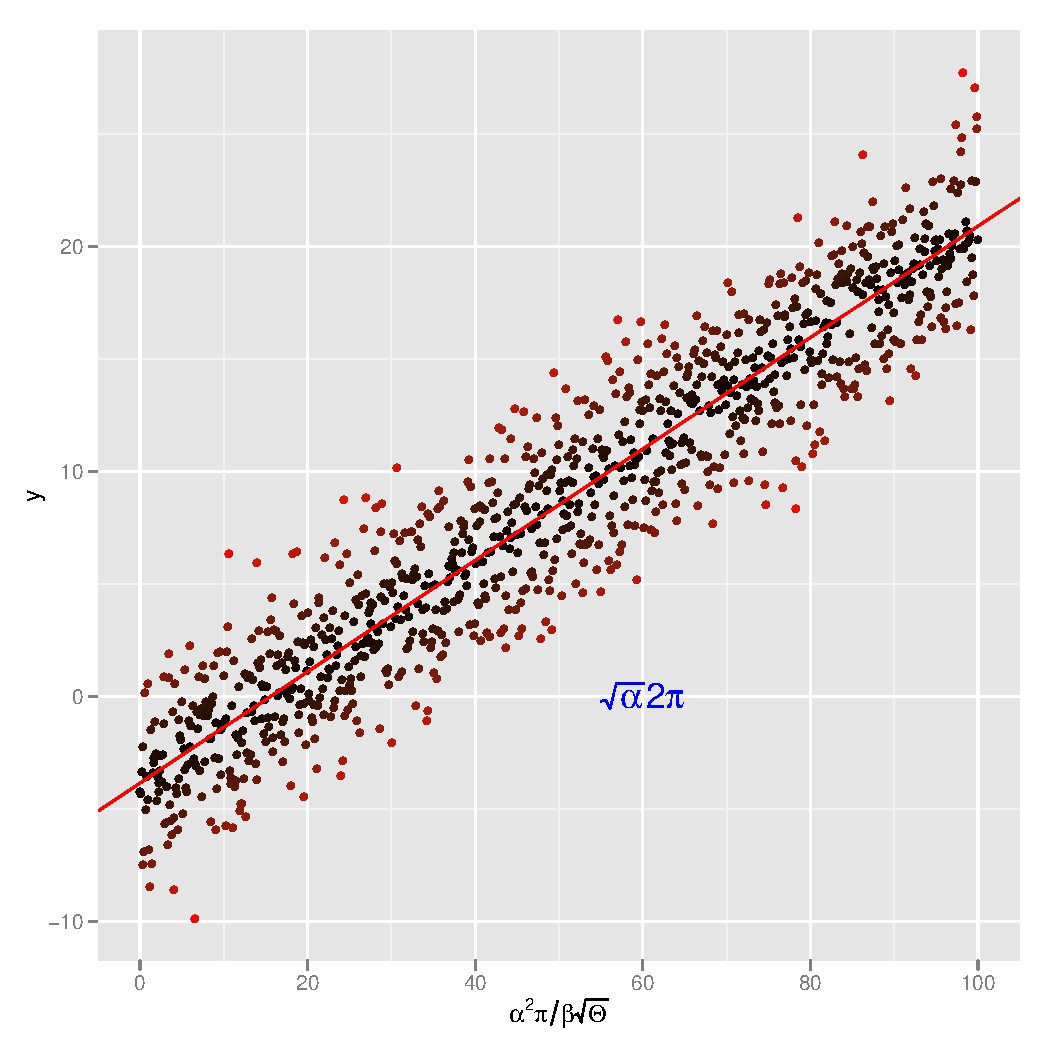
\includegraphics[width = .7\linewidth]{MyLinReg.pdf}
	\end{center}
	\caption{Linear regression with colors expressing residuals and
	mathematical annotations.}
	\label{LinReg}
\end{figure}

In Figure \ref{LinReg}, you can see the mathematical annotation on the
axis and in the plot area itself.

\subsection{\tt ggthemes}

The package {\tt ggthemes} provides you some additional {\tt geom}s, {\tt 
scale}s, and {\tt theme}s for {\tt ggplot}. These include a theme based 
on Tufte's {\it The Visual Display of Quantitative Information} (see 
the readings section at the end of this Chapter). First install the 
package:

\begin{lstlisting}
> install.packages("ggthemes")
\end{lstlisting}

Then try:

\begin{lstlisting}	
> library(ggthemes)

p <- ggplot(MyDF, aes(x = log(Predator.mass), y = log(Prey.mass),
				colour = Type.of.feeding.interaction )) +
				geom_point(size=I(2), shape=I(10)) + theme_bw()

> p + geom_rangeframe() + # now fine tune the geom to Tufte's range frame
		theme_tufte() # and theme to Tufte's minimal ink theme    
\end{lstlisting}

Go to \url{https://github.com/jrnold/ggthemes} for more 
information and a list of {\tt geom}s, {\tt theme}s, and {\tt scale}s. 

\begin{tipbox}
Both {\tt library()} and {\tt require()} are commands/functions to load 
packages. The difference is that {\tt require()} is designed for use 
inside other functions, so it returns {\tt FALSE} and gives a warning, 
whereas {\tt library()} returns an error by default if the package does 
not exist. 
\end{tipbox}

\section{Practicals} \label{sec:PPPrac2}
In this practical, you will write script that draws and saves a pdf 
file of Fig. \ref{PPRegress}, and writes the accompanying 
regression results to a formatted table in csv. Note that the plots 
show that the analysis must be subsetted by the {\tt 
Predator.lifestage} field of the dataset. The guidelines are:

\begin{compactitem}
		
	\item Write a {\tt R} script file called {\tt PP\_Regress.R} and save it in 
	the {\tt Code} directory --- sourcing or running this script should 
	result in one pdf file containing the following figure being 
	saved in the {\tt Results} directory:
	(Hint: Use the {\tt print()} command to write to the pdf)    
\end{compactitem}

\begin{figure}
	\begin{center}
				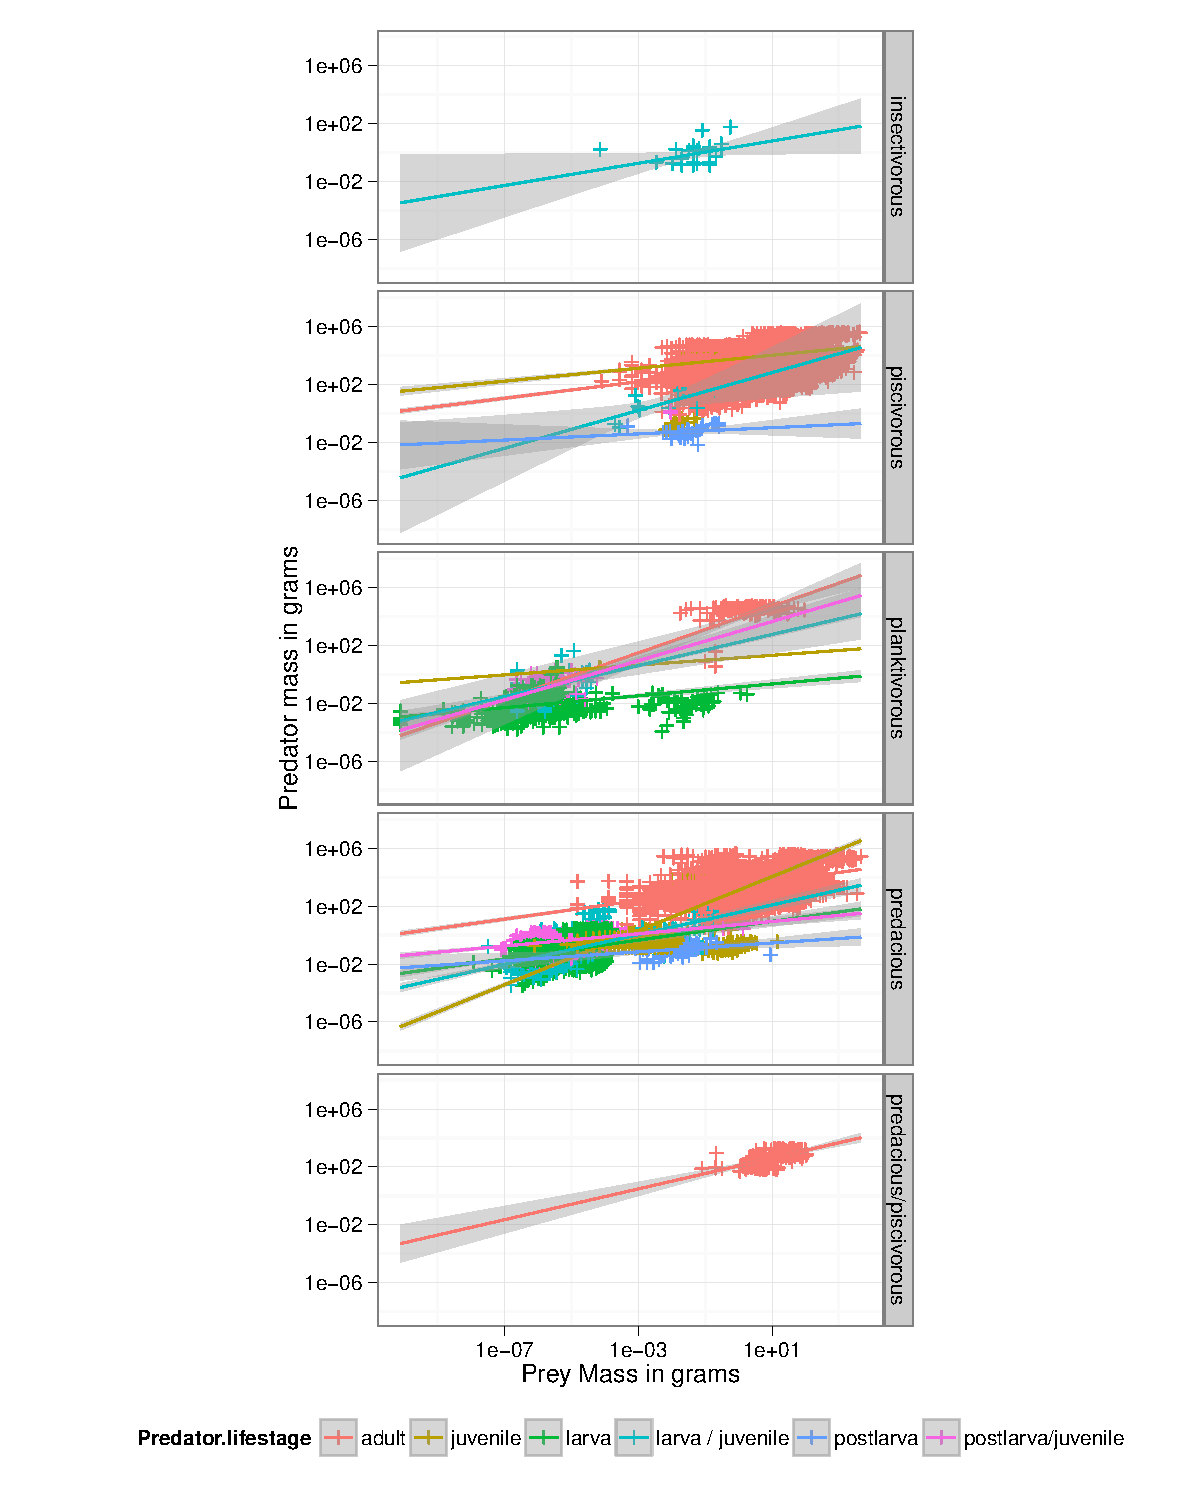
\includegraphics[scale=0.7]{Figure1.pdf}
	\end{center}
	\caption{Write a script that generates this figure}
	\label{PPRegress}
\end{figure}
	
\begin{compactitem}
	\item In addition, the script should calculate the regression results 
	corresponding to the lines fitted in the figure and save it to a csv 
	delimited table called ({\tt PP\_Regress\_Results.csv}), in the {\tt 
	Results} directory. (Hint: you will have to initialize a new 
	dataframe in the script to first store the calculations and then {\tt 
	write.csv()} or {\tt write.table()} it.) \\ 
	All that you are being asked for here is results of an analysis of 
	Linear regression on subsets of the data corresponding to available 
	Feeding Type $\times$ Predator life Stage combination --- not a 
	multivariate linear model with these two as separate covariates!

	\item The regression results should include the following with 
	appropriate headers (e.g., slope, intercept, etc, in each Feeding 
	type $\times$ life stage category): regression slope, regression 
	intercept, R$^2$, F-statistic value, and p-value of the overall 
	regression (Hint: Review the Stats week!).
 
 	\item The script should be self-sufficient and not need any 
	external inputs --- it should import the above predator-prey 
	dataset from the appropriate directory, and save the graphic plots 
	to the appropriate directory (Hint: use relative paths). I should 
	be able to {\tt source} it without errors.

	\item You can also use the {\tt dplyr} function instead of looping 
	(se Chapter \ref{chap:R_II}), and the {\tt ggplot} command 
	instead of {\tt qplot}.

\end{compactitem}

\noindent {\bf Extra Credit}: Do the same as above, but the analysis 
this time should be separate by the dataset's {\tt Location} field. 
Call it {\tt PP\_Regress\_loc.R}. No need to generate plots for this 
(just the analysis results to a {\tt *.csv} file), as a combination of 
{\tt Type.of.feeding.interaction}, {\tt Predator.lifestage}, and {\tt 
Location} will be far to busy (faceting by three variables is one step 
too far)!

\section{Data wrangling and exploration} 

You are likely to spend far more time than you think dredging through 
your data manually, checking it, editing it, and reformatting it to 
make it useful for the actual data exploration and statistical 
analysis. For example, you may need to:  
\begin{compactitem}
	\item Identify the variables vs observations within the data 
	--- somebody else might have recorded the data, or you might have 
	collected the data some time back!
	\item Fill in zeros (true measured/observed absences) 
	\item Identify and add a value (e.g., {\tt -999999}) to denote missing 
	observations	
	\item Derive or calculate new variables from the raw observations 
	(e.g., convert measurements to SI units; kilograms, meters, seconds, 
	etc.)
	\item Reshape/reformat your data into a layout that works best for 
	analysis (e.g., for {\tt R} itself) --- e.g., from wide to long data 
	format for repeated (across sites, plots, plates, chambers, etc) 
	measures data
	\item Merge multiple datasets together into a single data sheet
\end{compactitem}
And this is far from an exhaustive list. Doing so many different things 
to your raw data is both time-consuming and risky. Why risky? Because 
to err is very human, and every new, tired mouse-click and/or 
keyboard-stab has a high probability of being incorrect!  

\begin{figure}
	\begin{center}
    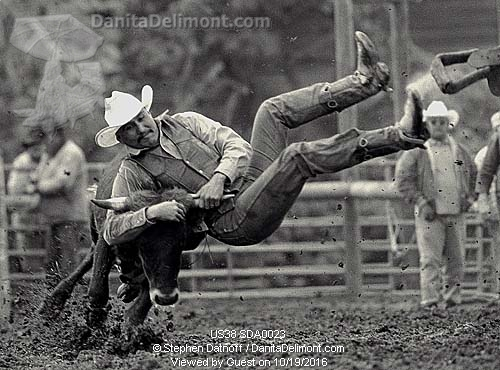
\includegraphics[width=.6\textwidth]{Wrangling2.jpg}
\end{center}
\caption{An illustration of a (metaphorical) datum being wrangled into submission.}
\end{figure}

\subsection{Some data wrangling principles} 
So you would like to a record of the data wrangling process (so that it 
is repeatable and even reversible), and automate it to the extent 
possible. To this end, here are some guidelines:

\begin{itemize}
	\item Store data in universally-readable, nonproprietary software formats (e.g., {\tt .csv})
	\item Use 
	plain ASCII text for your file names, variable/field/column names, and data 
	values --- make sure the ``text encoding'' is correct and standard 
	(e.g., {\tt UTF-8})
	\item Keep a metadata file for each unique dataset (agian, in 
	non-proprietary format)
	\item Don't (over-)modify your raw data by hand --- use scripts 
	instead --- keep a copy of the data as they were recorded.
	\item Use meaningful names for your data and files and field (column) names
	\item When you add data, try not to add columns (widening the format); rather, design your 
	tables/datasheets so that you add only rows (lengthening the format) 
	--- and convert ``wide format data'' to ``long format data'' using 
	scripts, not by hand!
	\item All cells within a data column should contain only one type of 
	information (i.e., either text (character), numeric, etc.). 
	\item Ultimately, consider creating a relational database for your 
	data (see the last section of this Chapter).
\end{itemize} 
This is not an exhaustive list either --- see the Borer et al (2009) 
paper in your readings list.

We will use the Pound Hill dataset collected by students in a past Silwood 
Field Course week for understanding/illustrating some of these 
principles. 

To start with, we need to import the {\tt raw} data file. 
\begin{compactitem}[$\quad\star$]
	\item Go to the bitbucket repository and navigate to the {\tt Data} 
	directory. 
	\item Copy the file {\tt PoundHillData.csv} and {\tt 
	PoundHillMetaData.csv} files into your own R module's {\tt
	Data} directory. 
	\item Now load the data in R: 
\end{compactitem}

\begin{lstlisting}
> MyData <- as.matrix(read.csv("../Data/PoundHillData.csv",header = F, 
stringsAsFactors = F))
> MyMetaData <- read.csv("../Data/PoundHillMetaData.csv",header = T, 
sep=";", stringsAsFactors = F)
\end{lstlisting}
Note that:
\begin{compactitem}
\item Loading the data {\tt as.matrix()}, and setting The {\tt header} 
and {\tt stringsAsFactors} guarantees that the data are imported "as 
is" so that you can wrangle them. Otherwise {\tt read.csv} will convert 
the first row to column headers, convert everything to factors, etc. 
Note that all the data will be converted to character class in matrix 
here because at least some of the entries are already character class.

\item For the metadata loading, the {\tt header} is set to true because 
we do have metadata headers ({\tt FieldName} and {\tt Description}), 
and I have used semicolon ({\tt ;}) as delimiter because there are 
commas in one of the field descriptions. 

\item I have avoided spaces in the columns headers (so ``FieldName'' 
instead of ``Field Name'') --- please avoid spaces in field or column 
names as much a possible as R will replace each space in a column 
header with a dot, which may be confusing.

\end{compactitem}

\begin{tipbox}
In {\tt R}, you can use {\tt F} and {\tt T} for boolean {\tt FALSE} 
and {\tt TRUE} respectively. Try:
\begin{lstlisting}
> a <- T
> a
[1] TRUE
\end{lstlisting}
\end{tipbox}

We won't do anything with the metadata file in this session except 
inspect the information it contains.   

\subsubsection{Keep a metadata file for each unique dataset} 

Data wrangling really begins immediately after data collection. You may 
collect data of different kinds (e.g., diversity, biomass, tree girth), 
etc. Keep the original spreadsheet well documented using a ``metadata'' 
file that describes the data (you would hopefully have written the 
first version of this even before you started collecting the data!). 
The minimum information needed to make a metadata file useful is a 
description of each of the {\it fields} --- the column or row headers 
under which the information is stored in your data/spreadsheet. Here is 
the metadata file for the Pound Hill dataset:
\begin{center}
	\begin{tabular}{|p{3.5cm} | p{11cm}|}
		\hline
		{\bf Field/Column Name} & {\bf Description} \\ \hline
		Cultivation	& Cultivation treatments applied in three months: october, may, march \\ \hline
		Block &	Treatment blocks ids: a--d \\ \hline
		Plot &	Plot ids under each treatment : 1--12 \\ \hline
		Quadrat	& Sampling quadrats (25$\times$50 cm each) per plot: Q1--Q6 
		\\ \hline
		Species	data & Number of individuals (count) per quadrat \\ \hline
	\end{tabular}
\end{center}

Ideally, you would also like to add more information about the data, 
such as the measurement units of each type of observation. Here, there 
is just one type of observation: Number of individuals of species per 
sample (plot), which is a count (integer, or {\tt int} class). 

\subsubsection{Don't (over-)modify your raw data by hand}

When the dataset is large (e.g., 1000's of rows), cleaning and 
exploring it can get tricky, and you are very likely to make many 
mistakes. You should record all the steps you used to process it with 
an R script rather than risking a manual and basically irreproducible 
processing. Most importantly {\it avoid or minimize editing your raw 
data file}. Let's see how we can modify the data using {\tt R}. In 
fact, we should now start to keep a record of what we are doing to the 
data. This is illustrated in a code data file available on the 
bitbucket repository. 

\begin{tipbox}
Sometimes you may run into (unexpected) bugs when importing and 
running scripts in {\tt R} because your file has a 
no-standard text encoding. You may need to specify the encoding in that 
case, using the {\tt encoding} argument of {\tt read.csv()} and {\tt 
read.table()}. You can check the encoding of a file by using {\tt find} in 
Linux/Mac. Try:
\begin{lstlisting}
$ file -i ../Data/PoundHillData.csv
\end{lstlisting}
or, check encoding of all files in the {\tt Data} directory: 
\begin{lstlisting}
$ file -i ../Data/*.csv 	
\end{lstlisting}
use {\tt file -I} instead of {\tt file -i} in a Mac terminal
\end{tipbox} 

\begin{compactitem}[$\quad\star$]
	\item Go to the bitbucket repository and navigate to the {\tt Code} 
	directory. 
	\item Copy the script {\tt DataWrang.R} into your own R module's {\tt 
	Code} directory and open it. 
\end{compactitem}

Go through the script carefully line by line, and make sure you 
understand what's going on. Read the comments --- add to them if you 
want. One of the examples of data modification that you must avoind 
doing by hand, is illustrated in the script: filling in zeros.  

\subsubsection{Convert wide format data to long format using scripts}

You typically record data in the field or experiments using a ``wide'' 
format, where a subject's (e.g., habitat, plot, treatment, species etc) 
repeated responses or observations (e.g., species count, biomass, etc) 
will be in a single row, and each response in a separate column. The 
raw Pound Hill data were recorded in precisely this way. However, the 
wide format is not ideal for data analysis --- instead you need the 
data in a ``long'' format, where each row is one observation point per 
subject. So each subject will have data in multiple rows. Any 
measures/variables/observations that don't change across the subjects 
will have the same value in all the rows.

\begin{tipbox}
For humans, the wide format is generally more intuitive for viewing and 
recording (e.g., in field data sheets) since one can actually view more 
of the data visually. However, the long format is more machine-readable 
and is closer to the formatting of databases. 
\end{tipbox}

You can switch between wide and formats using {\tt melt()} and {\tt 
dcast()} from the {\tt reshape2} package, as illustrated in {\tt DataWrang.R}. 

\subsection{And then came {\tt dplyr} and {\tt tidyr}}

So if you think this is the end of the options you have for data 
wrangling in R, think again. There are new kids on the block: {\tt dplyr} 
--- the next iteration of {\tt plyr} that addresses the speed issues in 
the latter, and {\tt tidyr}, essentially a nicer wrapper to the {\tt 
reshape2} package with additional functions. 
  
You will have to install these packages using {\tt sudo apt get 
install} in Linux or {\tt install.packages()} across all platforms (see 
Chapter \ref{chap:RI}). 

Together, these two packages have many many useful functions. Let's 
have a quick look at {\tt dplyr}:

\begin{lstlisting}
require(dplyr)
attach(iris)
dplyr::tbl_df(iris)	#like head(), but nicer!
dplyr::glimpse(iris) #like str(), but nicer!
utils::View(iris) #same as fix()!
dplyr::filter(iris, Sepal.Length > 7) #like subset(), but nicer!
dplyr::slice(iris, 10:15) # something new!
\end{lstlisting}

Note that the double colon ({\tt ::}) notation of {\tt dplyr} and {\tt 
tidyr} is like the dot notation in {\tt python} --- it allows you to 
access a particular function from these packages. So, for instance, if 
you want to use {\tt tbl\_df()} from {\tt dplyr}, the command syntax 
would be {\tt dplyr::tbl\_df(MyData)}. This new syntax is basically to 
avoid conflict in names of functions in by these new packages with the 
function names that already exist in the base R packages. For example, 
the {\tt dplyr} function {\tt filter} already exists in the base R 
package {\tt stats}. Thus, when you first load {dplyr}:  
\begin{lstlisting}	
> library(dplyr)
\end{lstlisting}	
you get:
\begin{lstlisting}	
Attaching package: 'dplyr'

The following objects are masked from 'package:stats':

    filter, lag

The following objects are masked from 'package:base':

    intersect, setdiff, setequal, union
\end{lstlisting}

Learning to use {\tt ddply} and {\tt tidyr} involves learning some new 
syntax and a lot of new commands, but if you plan to do a lot of data 
wrangling, you may want to get to know them well. Have a 
look at \url{https://blog.rstudio.org/2014/01/17/introducing-dplyr} and 
this cheatsheet: 
\url{https://www.rstudio.com/wp-content/uploads/2015/02/data-wrangling-cheatsheet.pdf}, also available in the Readings directory under {\tt DataDataData!} in 
the course bitbucket repository.

\subsection{On to data exploration}

Once you have wrangled the Pound Hill data to its long format, you are 
ready to go! You may want to start by examining the basic properties 
of the data, such as the number of tree species (41) in the dataset, 
number of quadrats (replicates) per plot and cultivation treatment, 
etc.

The first plot you can try is a histogram of abundances of species, 
grouped by different factors. For example, you can look at 
distributions of species' abundances grouped by {\tt Cultivation}). 

\section{Practicals}

{\bf (Extra Credit)} We used {\tt reshape2} in {\tt DataWrang.R} for 
wrangling that dataset. Write a new script called {\tt DataWrangTidy.R} 
that uses {\tt dplyr} and {\tt tidyr} for the same data wrangling 
steps. The best way to do this is to {\tt cp} {\tt DataWrang.R} and 
rename it {\tt DataWrangTidy.R}. Then systematically redo the script 
from start to end, looking for a function in {\tt dplyr} and {\tt 
tidyr} that does the same thing in each wrangling step. 

For example, to convert from wide to long format, instead of using {\tt 
melt()} (or {\tt dcast()}) from the {\tt reshape2} package, you can use  
{\tt gather()} from {\tt tidyr}.

Don't forget the cheatsheet: 
\url{https://www.rstudio.com/wp-content/uploads/2015/02/data-wrangling-cheatsheet.pdf} 
(also available in the Readings directory under {\tt DataDataData!} in 
the course bitbucket repository).

\section{Handling Big Data in R}

The  buzzword `Big Data' basically refers to datasets that have the 
following properties:
\begin{enumerate}

\item A dataset that does not fit into available RAM on one system 
(say, > 2 gigabytes). 
\item A dataset that has so many rows (when in it's long format --- see 
above sections) that it significantly slows down your analysis or 
simulation without vectorization (that is, when looping).	
\end{enumerate} 

Both these criteria are programming language- and computer 
hardware-dependent, of course. For example, a 32-bit OS can only handle 
$\textasciitilde$2 GB of RAM, so your computer screams ``Big Data!'' (slows down/hangs) 
every time you try to handle a dataset in that range. 

R reads data into RAM all at once when you using the {\tt read.table} 
(or its wrapper, {\tt read.csv()} --- maybe you have realized by now 
that {\tt read.csv()} is basically calling {\tt read.table()} with a 
particular set of options. That is, objects in R live in memory 
entirely, and big-ish data in RAM will cause R to choke. Python has 
similar problems, but you can circumvent these to an extent by using 
{\tt numpy} arrays (Chapter \ref{chap:pythonII}).

There are a few options (which you can combine, of course) if you 
are actually using datasets that are so large:

\begin{itemize}
	\item Import large files smartly; e.g., using {\tt scan()} in R, and 
	then create subsets of the data that you need. Also, use the {\tt 
	reshape} or {\tt tidyr} package to covert your data in the most 
	``square'' (so neither too long or too wide) format as possible. Of 
	course, you will need subsets of data in long format for analysis 
	(see sections above).
	\item use the {\tt bigmemory} package to load data in the gb range (e.g., use 
	{\tt read.big.matrix()} instead of {\tt read.table()}. This package 
	also has other useful functions, such as {\tt foreach()} instead of 
	{\tt for()} for better memory management. 
	\item Use a 64 bit version of R with enough memory and preferably on 
	Linux!
	\item Vectorize your analyses/simulations to the extent possible 
	(Chapters \ref{chap:pythonII}, \ref{chap:R_II}). 
	\item Use databases.
	\item use distributed computing (distribute the analysis/simulation 
	across multiple CPU's).
\end{itemize}
 
The next subsection superficially covers databases. We will cover 
memory management in the advanced Python, HPC and C weeks.

\subsection{Databases and R}

R can be used to link to and extract data from online databases such as PubMed 
and GenBank, or to manipulate and access your own. 
Computational Biology datasets are often quite 
large, and it makes sense to access their data by querying the 
databases instead of manually downloading them. So also, your own data 
may be complex and large, in which case you may want to organize and 
manage those data in a proper relational database. 

Practically all the data wrangling principles in the previous sections 
are a part and parcel of relational databases. 

There are many R packages 
that provide an interface to databases (SQLite, MySQL, Oracle, etc). 
Check out R packages {\tt DBI} 
(\url{http://cran.r-project.org/web/packages/DBI/index.html}) and {\tt 
RMySQL} 
(\url{https://cran.r-project.org/web/packages/RMySQL/index.html}.

And just like python (see Chapter \ref{chap:pythonII}), R can also be used 
to access, update and manage databases. In particular {\tt SQLite} 
allows you to build, manipulate, and access databases easily. Try this script 
(available in the {\tt Code} directory of the master repo):
\lstinputlisting[language=R]{Practicals/Code/SQLinR.R} 
This assumes that you are already familiar with the databases section 
of Chapter \ref{chap:pythonII}. 

\section{Practicals wrap-up}

  \begin{enumerate}

	\item Review and make sure you can run all the commands, code 
	fragments, and named scripts we have built till now and get the 
	expected outputs.

	\item Annotate/comment your code lines as much and as often as necessary 
	using \#.
	
	\item Keep all code, data and results files organized in you R 
	module directory
	 
   \end{enumerate}

\begin{center}
	\it {\tt git add}, {\tt commit} and {\tt push} all your code and data 
	from this chapter to your git repository.
\end{center}

\section{Readings}
Check out {\tt DataDataData!}, {\tt Visualization} and {\tt R} under 
{\tt Readings} on the bitbucket master repository
\begin{itemize}
   
  \item Brian McGill's ``Ten commandments for good data management''; \url{https://dynamicecology.wordpress.com/2016/08/22/ten-commandments-for-good-data-management/}

  \item This paper covers similar ground (look in your readings 
  directory): Borer, E. T., Seabloom, E. W., Jones, M. B., \& 
  Schildhauer, M. (2009). Some Simple Guidelines for Effective Data 
  Management. Bulletin of the Ecological Society of America, 90(2), 
  205--214.
  
  \item wrangler: \url{http://vis.stanford.edu/papers/wrangler}

  \item An interactive framework for data cleaning: \url{https://www2.eecs.berkeley.edu/Pubs/TechRpts/2000/CSD-00-1110.pdf}

  \item \url{http://www.theanalysisfactor.com/wide-and-long-data/}

	\item Rolandi et al. ``A Brief Guide to Designing Effective
	Figures for the Scientific Paper'', doi:10.1002/adma.201102518

	\item The classic Tufte \url{www.edwardtufte.com/tufte/books\_vdqi}

   Available in the Central Library, I have also added extracts and a 
    related book in pdf on the master repository

		(btw, check out what Tufte thinks of PowerPoint; \url{ https://www.edwardtufte.com/tufte/powerpoint})\\

	\item Lauren {\tt et al.} ``Graphs, Tables, and Figures in
	Scientific Publications: The Good, the Bad, and How Not to Be the
	Latter'', doi:10.1016/j.jhsa.2011.12.041

  \item Effective scientific illustrations: 
    \url{www.labtimes.org/labtimes/issues/lt2008/lt05/lt\_2008\_05\_52\_53.pdf} 

  \item 
    \url{https://web.archive.org/web/20120310121708/http://addictedtor.free.fr/graphiques/thumbs.php}

\end{itemize}
